\documentclass[11pt]{article}
\usepackage[textwidth=18.0cm, textheight=23.0cm, top=2.0cm]{geometry}
\usepackage{pst-all}
\usepackage{amssymb}
\usepackage{tikz}
\usepackage{underscore}\begin{document}
\pagestyle{empty}


ClassName: \underline{\textbf{Class_08.2bp-48}}
\par
BinSize: \underline{\textbf{100 × 100}}
\par
ReduceSize: \underline{\textbf{100 × 100}}
\par
TypeNum: \underline{\textbf{99}}
\par
Num: \underline{\textbf{100}}
\par
OutS: \underline{\textbf{270000}}
\par
InS: \underline{\textbf{234344}}
\par
Rate: \underline{\textbf{0.868}}
\par
UB: \underline{\textbf{27}}
\par
LB0: \underline{\textbf{27}}
\par
LB: \underline{\textbf{27}}
\par
LBWithCut: \underline{\textbf{27}}
\par
NodeCut: \underline{\textbf{0}}
\par
ExtendedNodeCnt: \underline{\textbf{1}}
\par
GenNodeCnt: \underline{\textbf{1}}
\par
PrimalNode: \underline{\textbf{0}}
\par
ColumnCount: \underline{\textbf{27}}
\par
TotalCutCount: \underline{\textbf{0}}
\par
RootCutCount: \underline{\textbf{0}}
\par
LPSolverCnt: \underline{\textbf{1}}
\par
PricingSolverCnt: \underline{\textbf{0}}
\par
BranchAndBoundNum: \underline{\textbf{1}}
\par
isOpt: \underline{\textbf{true}}
\par
TimeOnInitSolution: \underline{\textbf{0.440 s}}
\par
TimeOnPrimal: \underline{\textbf{0.000 s}}
\par
TimeOnPricing: \underline{\textbf{0.000 s}}
\par
TimeOnRmp: \underline{\textbf{0.078 s}}
\par
TotalTime: \underline{\textbf{0.581 s}}
\par
\newpage


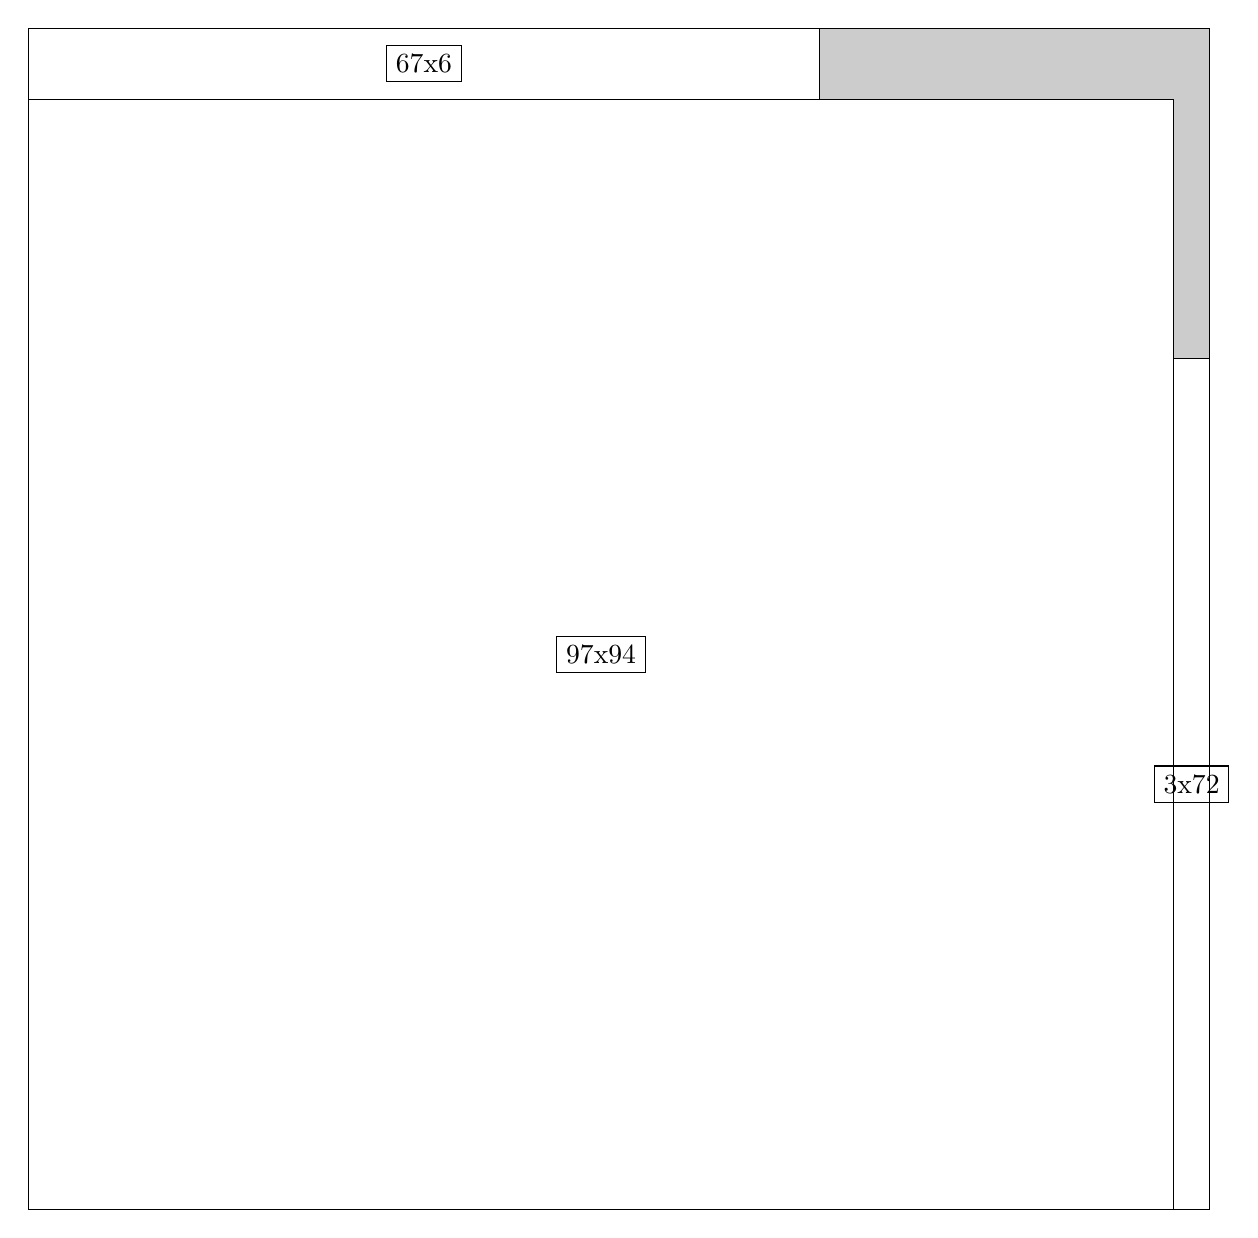
\begin{tikzpicture}[shorten >=1pt,scale=1.0,every node/.style={scale=1.0},->]
\tikzstyle{vertex}=[circle,fill=black!25,minimum size=14pt,inner sep=0pt]
\filldraw[fill=gray!40!white, draw=black] (0,0) rectangle (15.0,15.0);
\foreach \name/\x/\y/\w/\h in {97x94/0.0/0.0/14.549999999999999/14.1,67x6/0.0/14.1/10.049999999999999/0.8999999999999999,3x72/14.549999999999999/0.0/0.44999999999999996/10.799999999999999}
\filldraw[fill=white!40!white, draw=black] (\x,\y) rectangle node[draw] (\name) {\name} ++(\w,\h);
\end{tikzpicture}


w =97 , h =94 , x =0 , y =0 , v =9118
\par
w =67 , h =6 , x =0 , y =94 , v =402
\par
w =3 , h =72 , x =97 , y =0 , v =216
\par
\newpage


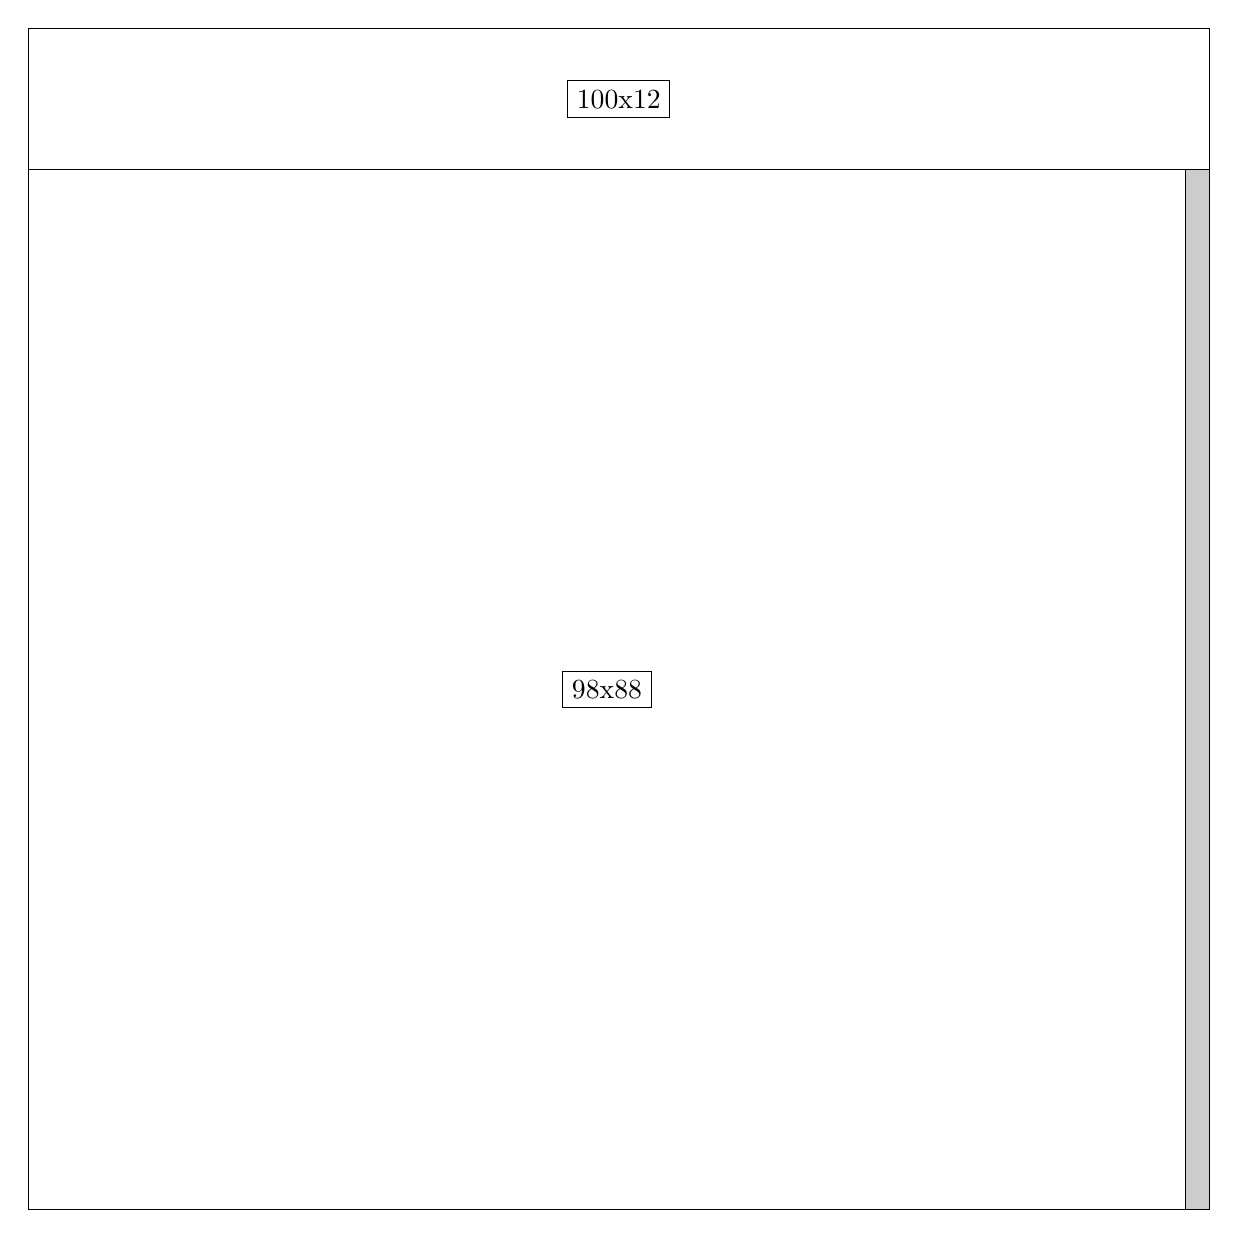
\begin{tikzpicture}[shorten >=1pt,scale=1.0,every node/.style={scale=1.0},->]
\tikzstyle{vertex}=[circle,fill=black!25,minimum size=14pt,inner sep=0pt]
\filldraw[fill=gray!40!white, draw=black] (0,0) rectangle (15.0,15.0);
\foreach \name/\x/\y/\w/\h in {98x88/0.0/0.0/14.7/13.2,100x12/0.0/13.2/15.0/1.7999999999999998}
\filldraw[fill=white!40!white, draw=black] (\x,\y) rectangle node[draw] (\name) {\name} ++(\w,\h);
\end{tikzpicture}


w =98 , h =88 , x =0 , y =0 , v =8624
\par
w =100 , h =12 , x =0 , y =88 , v =1200
\par
\newpage


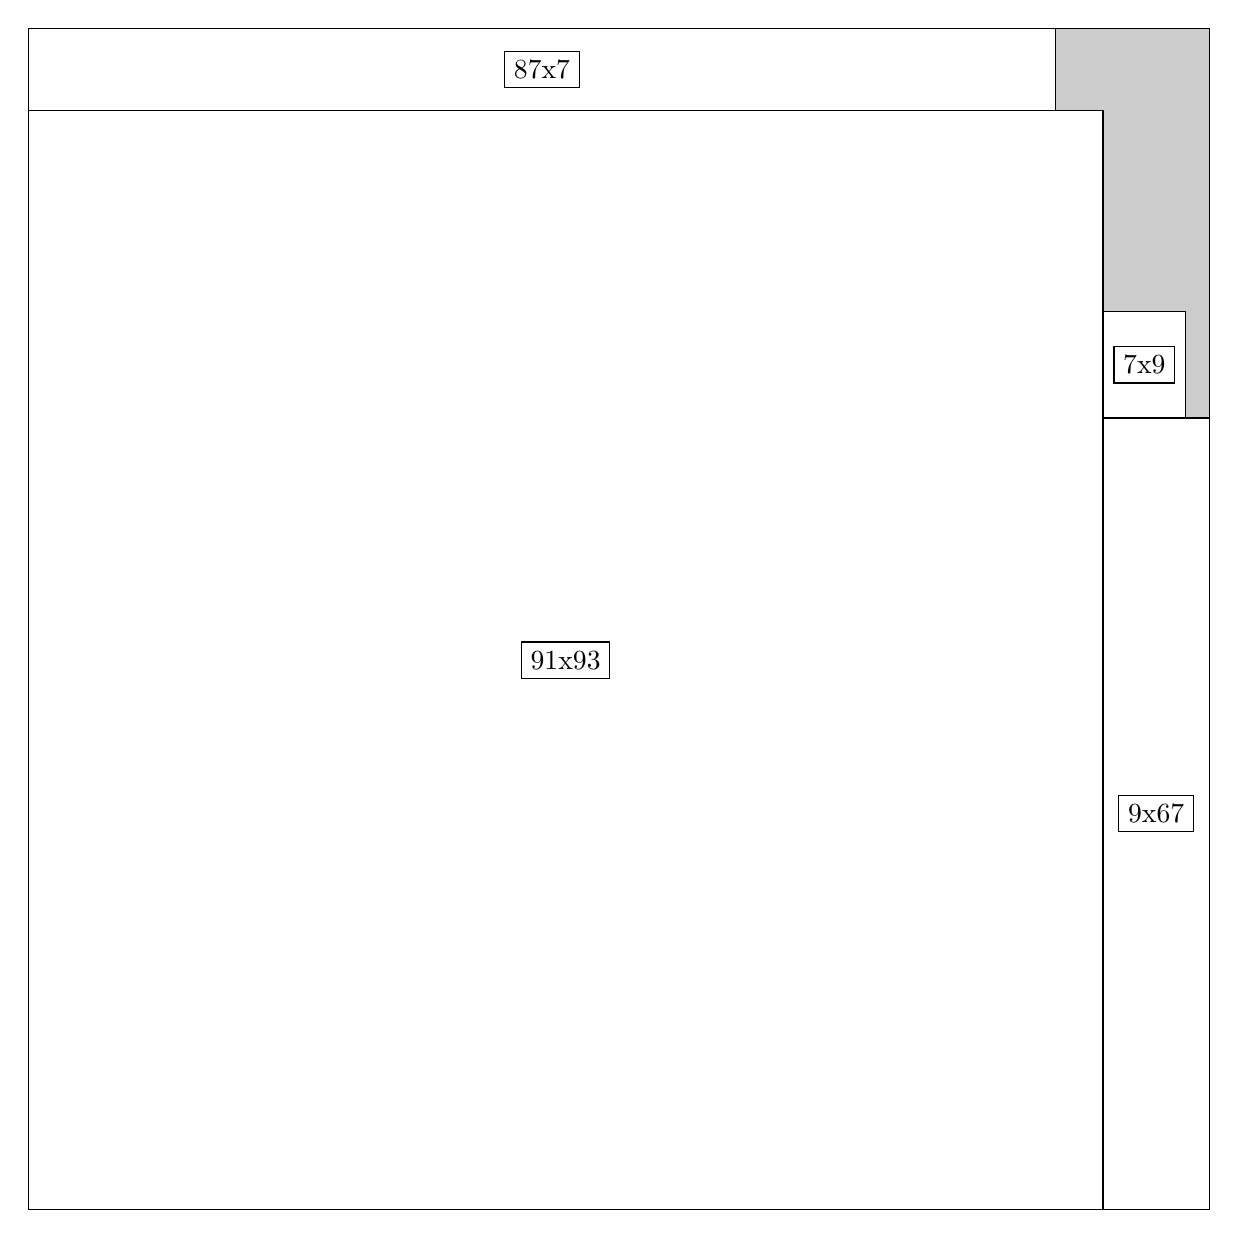
\begin{tikzpicture}[shorten >=1pt,scale=1.0,every node/.style={scale=1.0},->]
\tikzstyle{vertex}=[circle,fill=black!25,minimum size=14pt,inner sep=0pt]
\filldraw[fill=gray!40!white, draw=black] (0,0) rectangle (15.0,15.0);
\foreach \name/\x/\y/\w/\h in {91x93/0.0/0.0/13.65/13.95,87x7/0.0/13.95/13.049999999999999/1.05,9x67/13.65/0.0/1.3499999999999999/10.049999999999999,7x9/13.65/10.049999999999999/1.05/1.3499999999999999}
\filldraw[fill=white!40!white, draw=black] (\x,\y) rectangle node[draw] (\name) {\name} ++(\w,\h);
\end{tikzpicture}


w =91 , h =93 , x =0 , y =0 , v =8463
\par
w =87 , h =7 , x =0 , y =93 , v =609
\par
w =9 , h =67 , x =91 , y =0 , v =603
\par
w =7 , h =9 , x =91 , y =67 , v =63
\par
\newpage


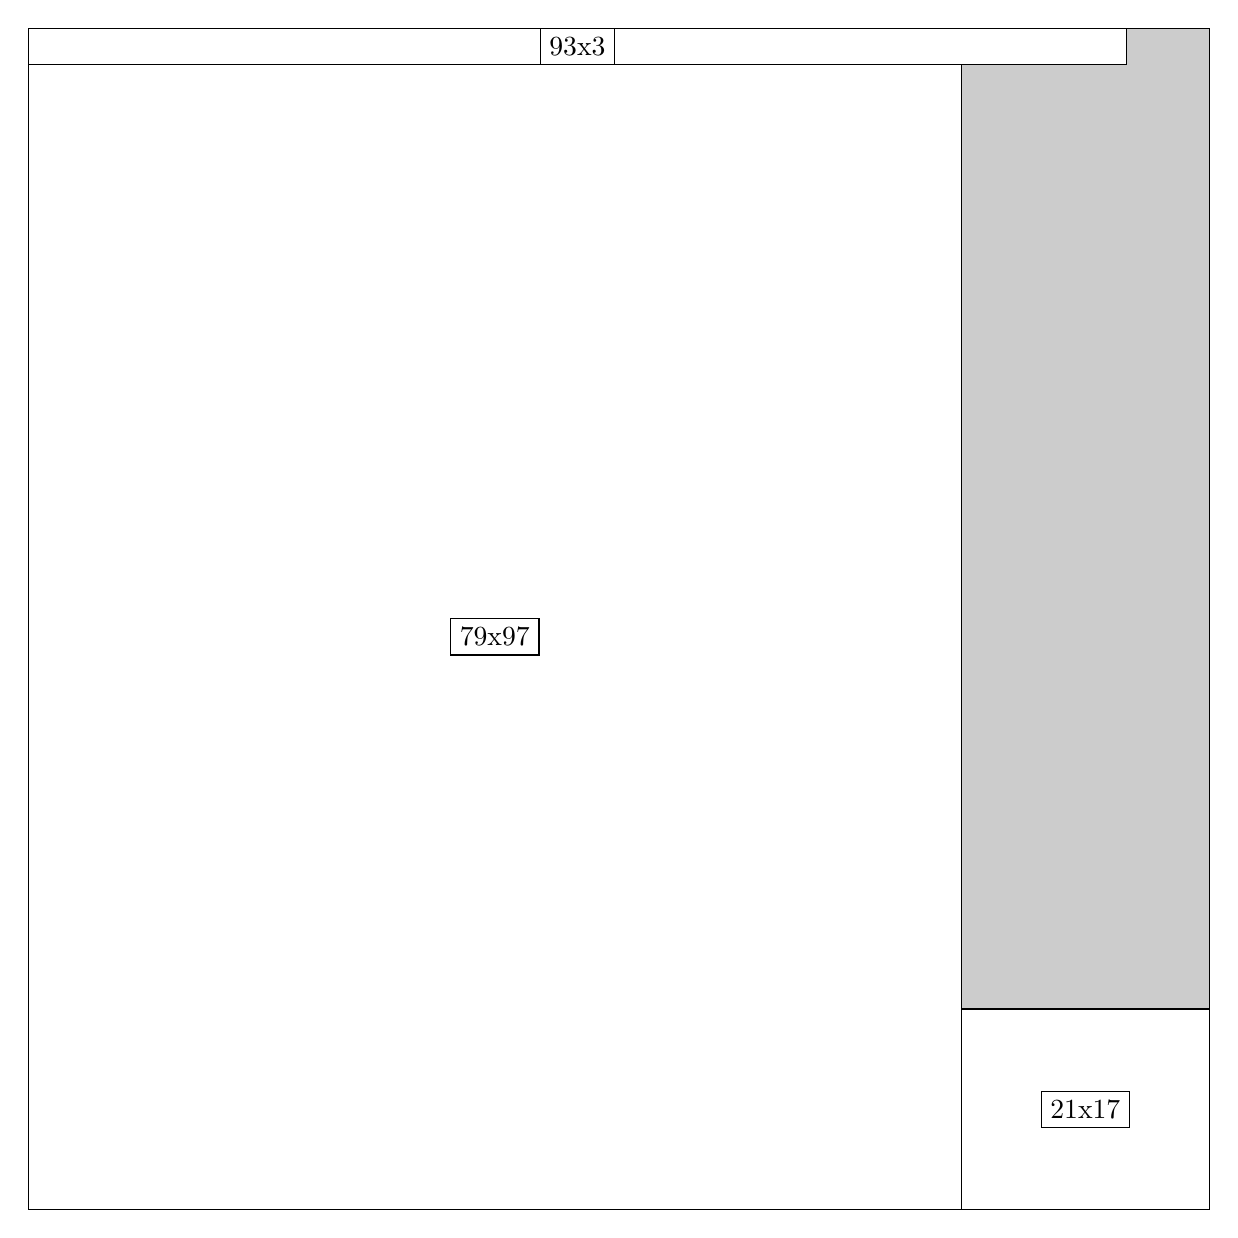
\begin{tikzpicture}[shorten >=1pt,scale=1.0,every node/.style={scale=1.0},->]
\tikzstyle{vertex}=[circle,fill=black!25,minimum size=14pt,inner sep=0pt]
\filldraw[fill=gray!40!white, draw=black] (0,0) rectangle (15.0,15.0);
\foreach \name/\x/\y/\w/\h in {79x97/0.0/0.0/11.85/14.549999999999999,21x17/11.85/0.0/3.15/2.55,93x3/0.0/14.549999999999999/13.95/0.44999999999999996}
\filldraw[fill=white!40!white, draw=black] (\x,\y) rectangle node[draw] (\name) {\name} ++(\w,\h);
\end{tikzpicture}


w =79 , h =97 , x =0 , y =0 , v =7663
\par
w =21 , h =17 , x =79 , y =0 , v =357
\par
w =93 , h =3 , x =0 , y =97 , v =279
\par
\newpage


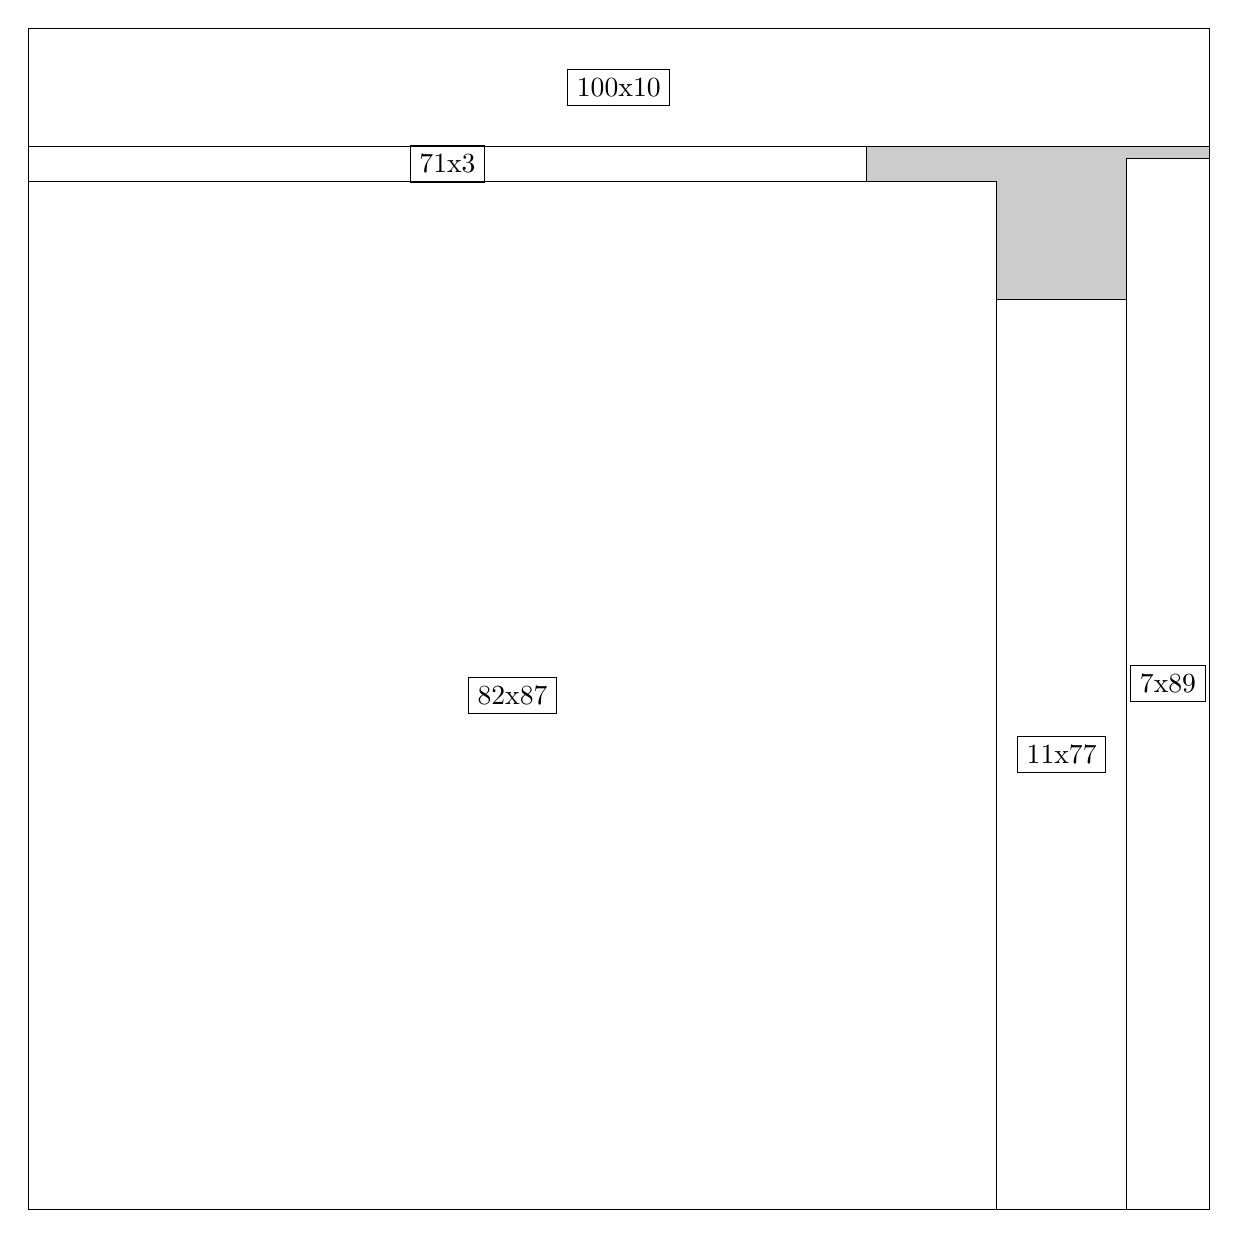
\begin{tikzpicture}[shorten >=1pt,scale=1.0,every node/.style={scale=1.0},->]
\tikzstyle{vertex}=[circle,fill=black!25,minimum size=14pt,inner sep=0pt]
\filldraw[fill=gray!40!white, draw=black] (0,0) rectangle (15.0,15.0);
\foreach \name/\x/\y/\w/\h in {82x87/0.0/0.0/12.299999999999999/13.049999999999999,100x10/0.0/13.5/15.0/1.5,11x77/12.299999999999999/0.0/1.65/11.549999999999999,7x89/13.95/0.0/1.05/13.35,71x3/0.0/13.049999999999999/10.65/0.44999999999999996}
\filldraw[fill=white!40!white, draw=black] (\x,\y) rectangle node[draw] (\name) {\name} ++(\w,\h);
\end{tikzpicture}


w =82 , h =87 , x =0 , y =0 , v =7134
\par
w =100 , h =10 , x =0 , y =90 , v =1000
\par
w =11 , h =77 , x =82 , y =0 , v =847
\par
w =7 , h =89 , x =93 , y =0 , v =623
\par
w =71 , h =3 , x =0 , y =87 , v =213
\par
\newpage


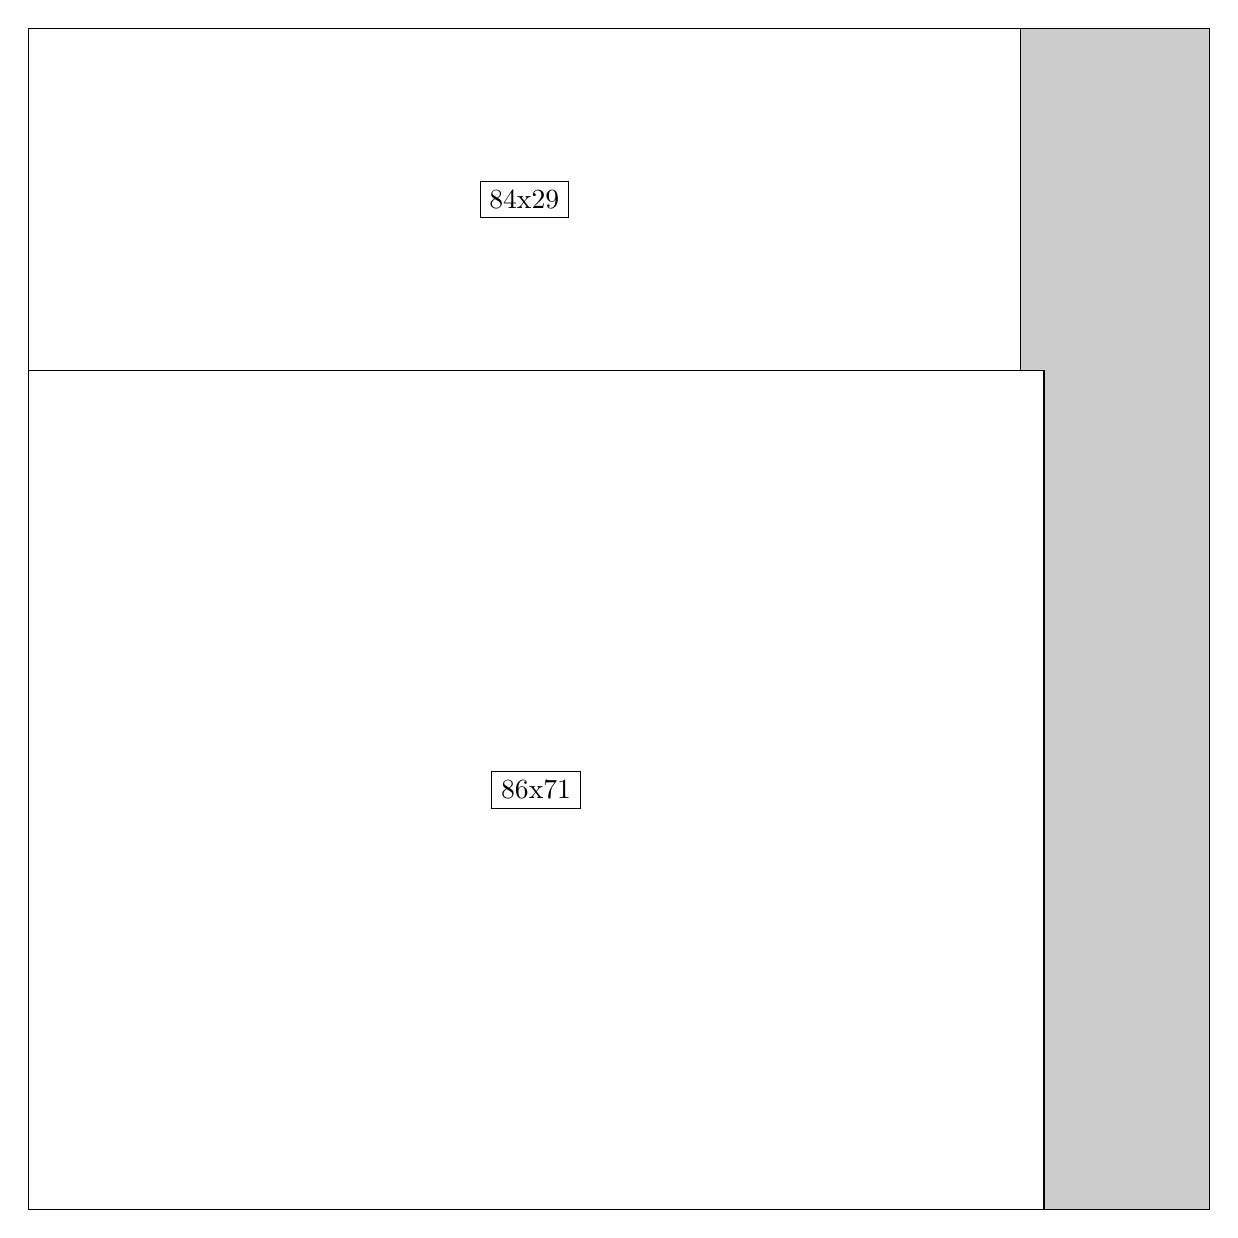
\begin{tikzpicture}[shorten >=1pt,scale=1.0,every node/.style={scale=1.0},->]
\tikzstyle{vertex}=[circle,fill=black!25,minimum size=14pt,inner sep=0pt]
\filldraw[fill=gray!40!white, draw=black] (0,0) rectangle (15.0,15.0);
\foreach \name/\x/\y/\w/\h in {86x71/0.0/0.0/12.9/10.65,84x29/0.0/10.65/12.6/4.35}
\filldraw[fill=white!40!white, draw=black] (\x,\y) rectangle node[draw] (\name) {\name} ++(\w,\h);
\end{tikzpicture}


w =86 , h =71 , x =0 , y =0 , v =6106
\par
w =84 , h =29 , x =0 , y =71 , v =2436
\par
\newpage


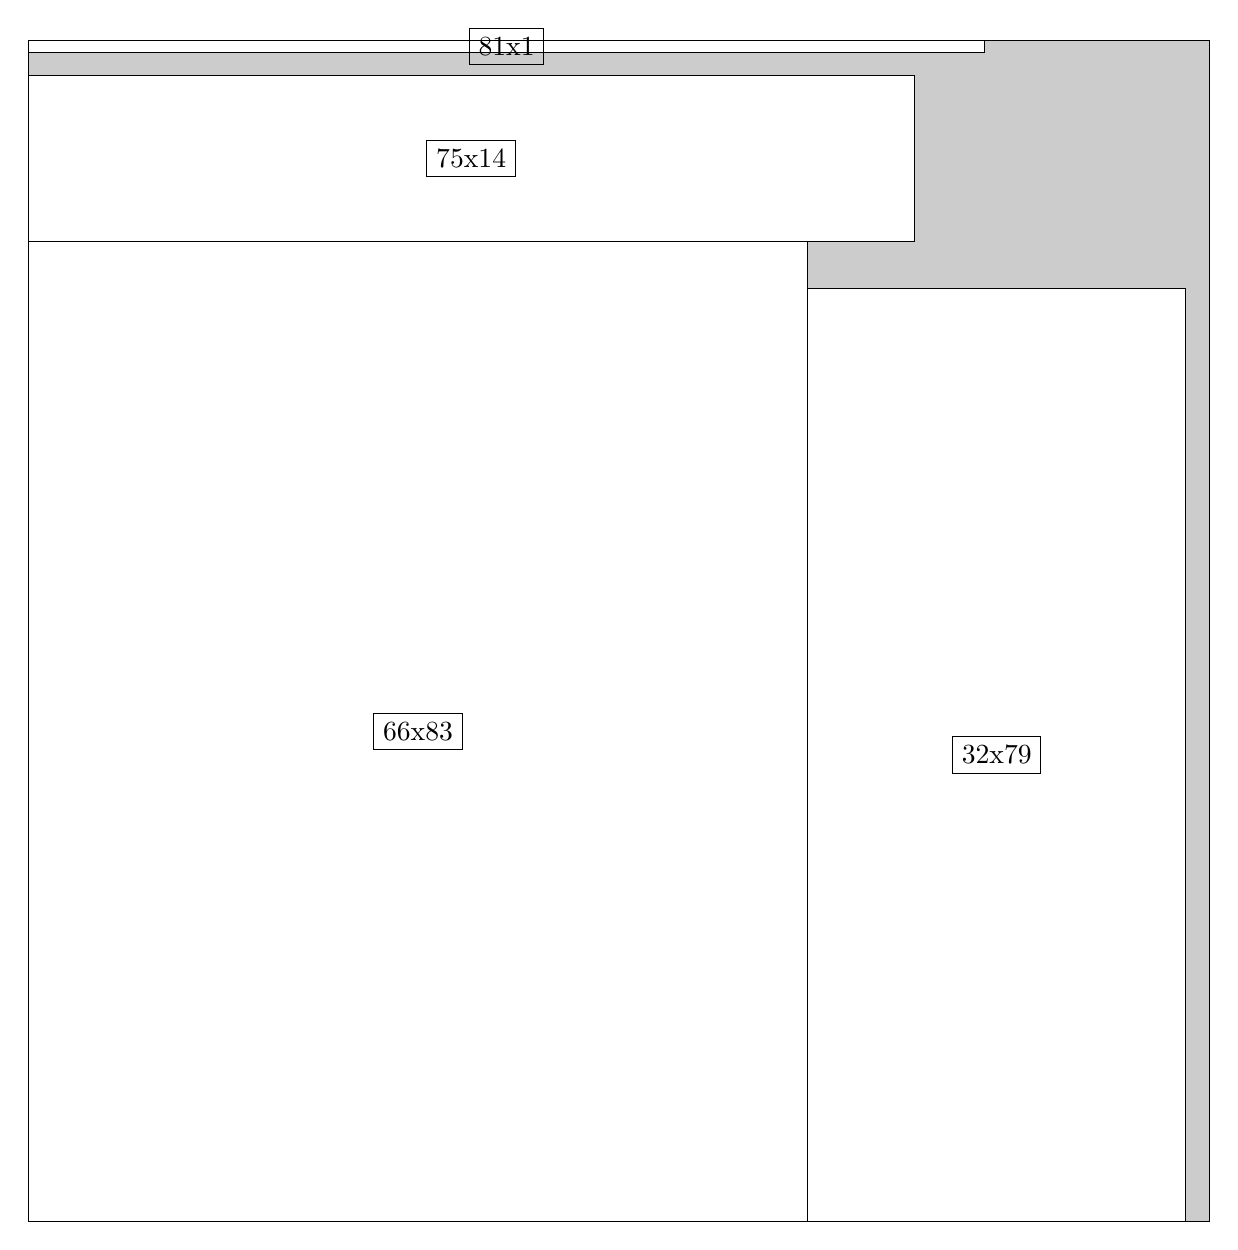
\begin{tikzpicture}[shorten >=1pt,scale=1.0,every node/.style={scale=1.0},->]
\tikzstyle{vertex}=[circle,fill=black!25,minimum size=14pt,inner sep=0pt]
\filldraw[fill=gray!40!white, draw=black] (0,0) rectangle (15.0,15.0);
\foreach \name/\x/\y/\w/\h in {66x83/0.0/0.0/9.9/12.45,32x79/9.9/0.0/4.8/11.85,75x14/0.0/12.45/11.25/2.1,81x1/0.0/14.85/12.15/0.15}
\filldraw[fill=white!40!white, draw=black] (\x,\y) rectangle node[draw] (\name) {\name} ++(\w,\h);
\end{tikzpicture}


w =66 , h =83 , x =0 , y =0 , v =5478
\par
w =32 , h =79 , x =66 , y =0 , v =2528
\par
w =75 , h =14 , x =0 , y =83 , v =1050
\par
w =81 , h =1 , x =0 , y =99 , v =81
\par
\newpage


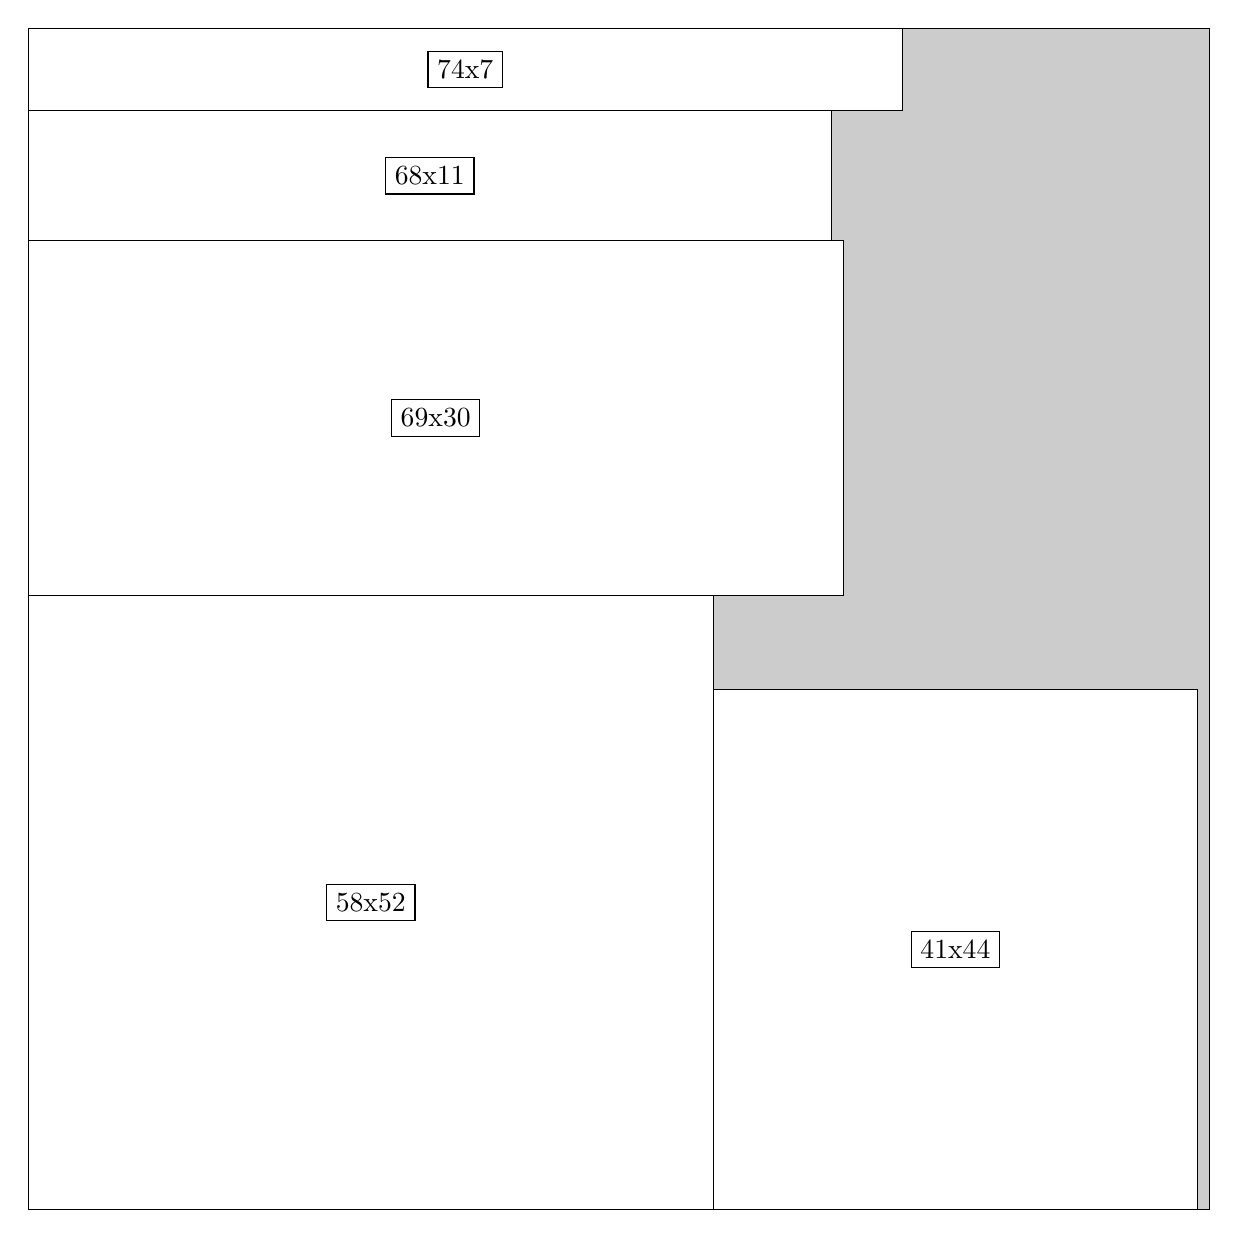
\begin{tikzpicture}[shorten >=1pt,scale=1.0,every node/.style={scale=1.0},->]
\tikzstyle{vertex}=[circle,fill=black!25,minimum size=14pt,inner sep=0pt]
\filldraw[fill=gray!40!white, draw=black] (0,0) rectangle (15.0,15.0);
\foreach \name/\x/\y/\w/\h in {41x44/8.7/0.0/6.1499999999999995/6.6,69x30/0.0/7.8/10.35/4.5,58x52/0.0/0.0/8.7/7.8,68x11/0.0/12.299999999999999/10.2/1.65,74x7/0.0/13.95/11.1/1.05}
\filldraw[fill=white!40!white, draw=black] (\x,\y) rectangle node[draw] (\name) {\name} ++(\w,\h);
\end{tikzpicture}


w =41 , h =44 , x =58 , y =0 , v =1804
\par
w =69 , h =30 , x =0 , y =52 , v =2070
\par
w =58 , h =52 , x =0 , y =0 , v =3016
\par
w =68 , h =11 , x =0 , y =82 , v =748
\par
w =74 , h =7 , x =0 , y =93 , v =518
\par
\newpage


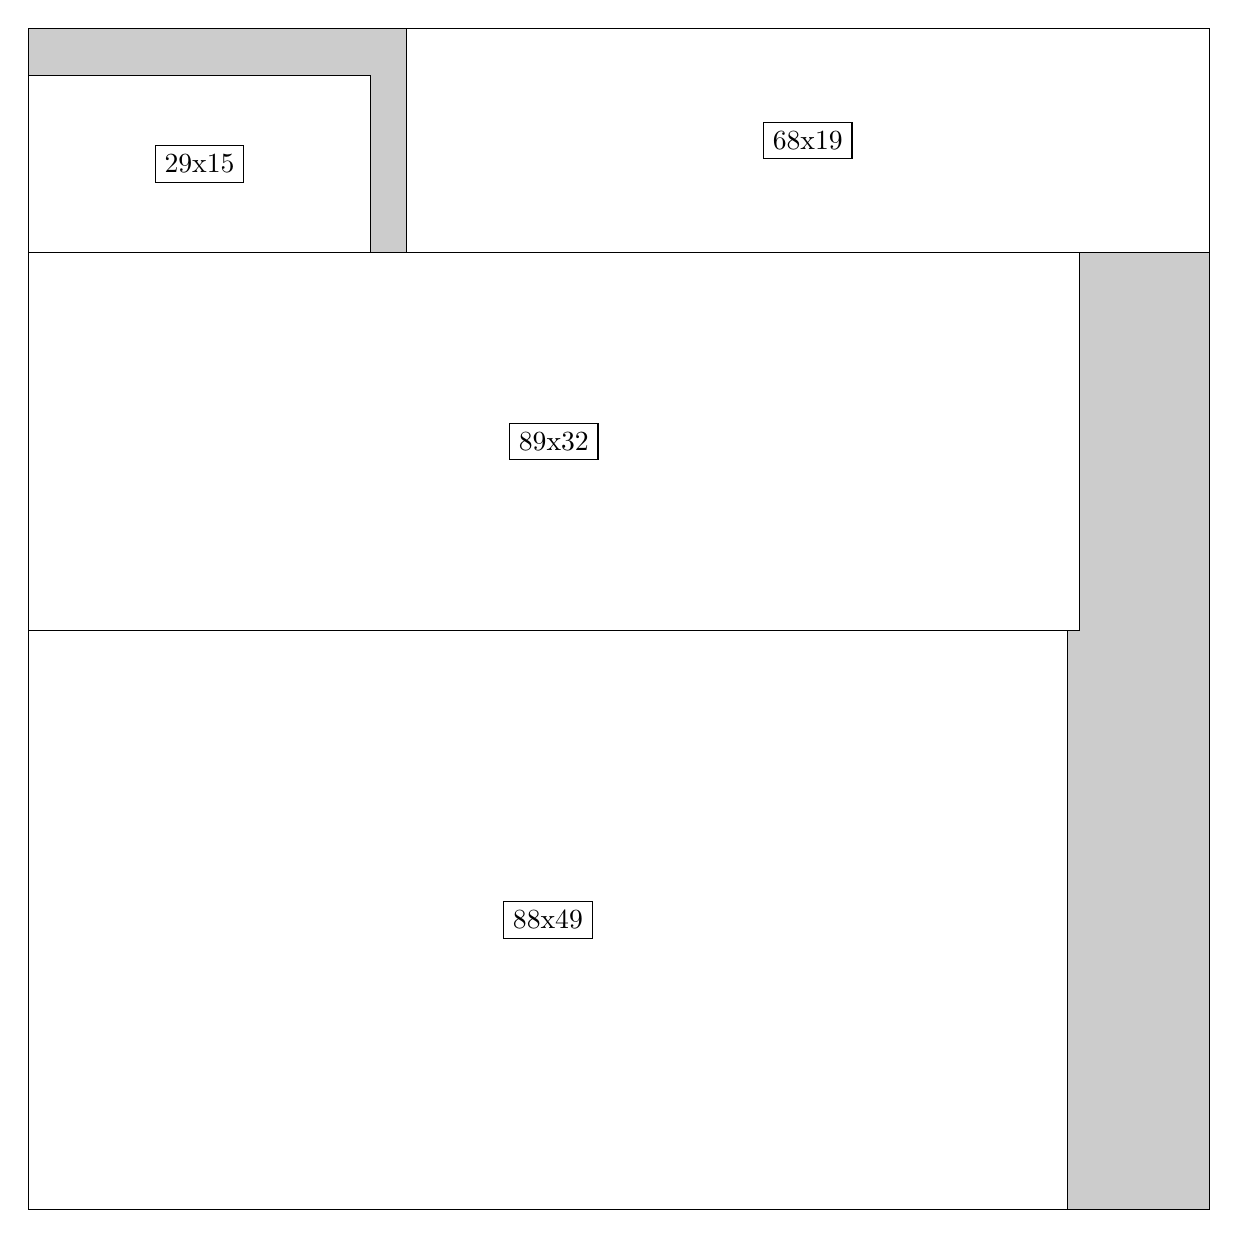
\begin{tikzpicture}[shorten >=1pt,scale=1.0,every node/.style={scale=1.0},->]
\tikzstyle{vertex}=[circle,fill=black!25,minimum size=14pt,inner sep=0pt]
\filldraw[fill=gray!40!white, draw=black] (0,0) rectangle (15.0,15.0);
\foreach \name/\x/\y/\w/\h in {88x49/0.0/0.0/13.2/7.35,89x32/0.0/7.35/13.35/4.8,68x19/4.8/12.15/10.2/2.85,29x15/0.0/12.15/4.35/2.25}
\filldraw[fill=white!40!white, draw=black] (\x,\y) rectangle node[draw] (\name) {\name} ++(\w,\h);
\end{tikzpicture}


w =88 , h =49 , x =0 , y =0 , v =4312
\par
w =89 , h =32 , x =0 , y =49 , v =2848
\par
w =68 , h =19 , x =32 , y =81 , v =1292
\par
w =29 , h =15 , x =0 , y =81 , v =435
\par
\newpage


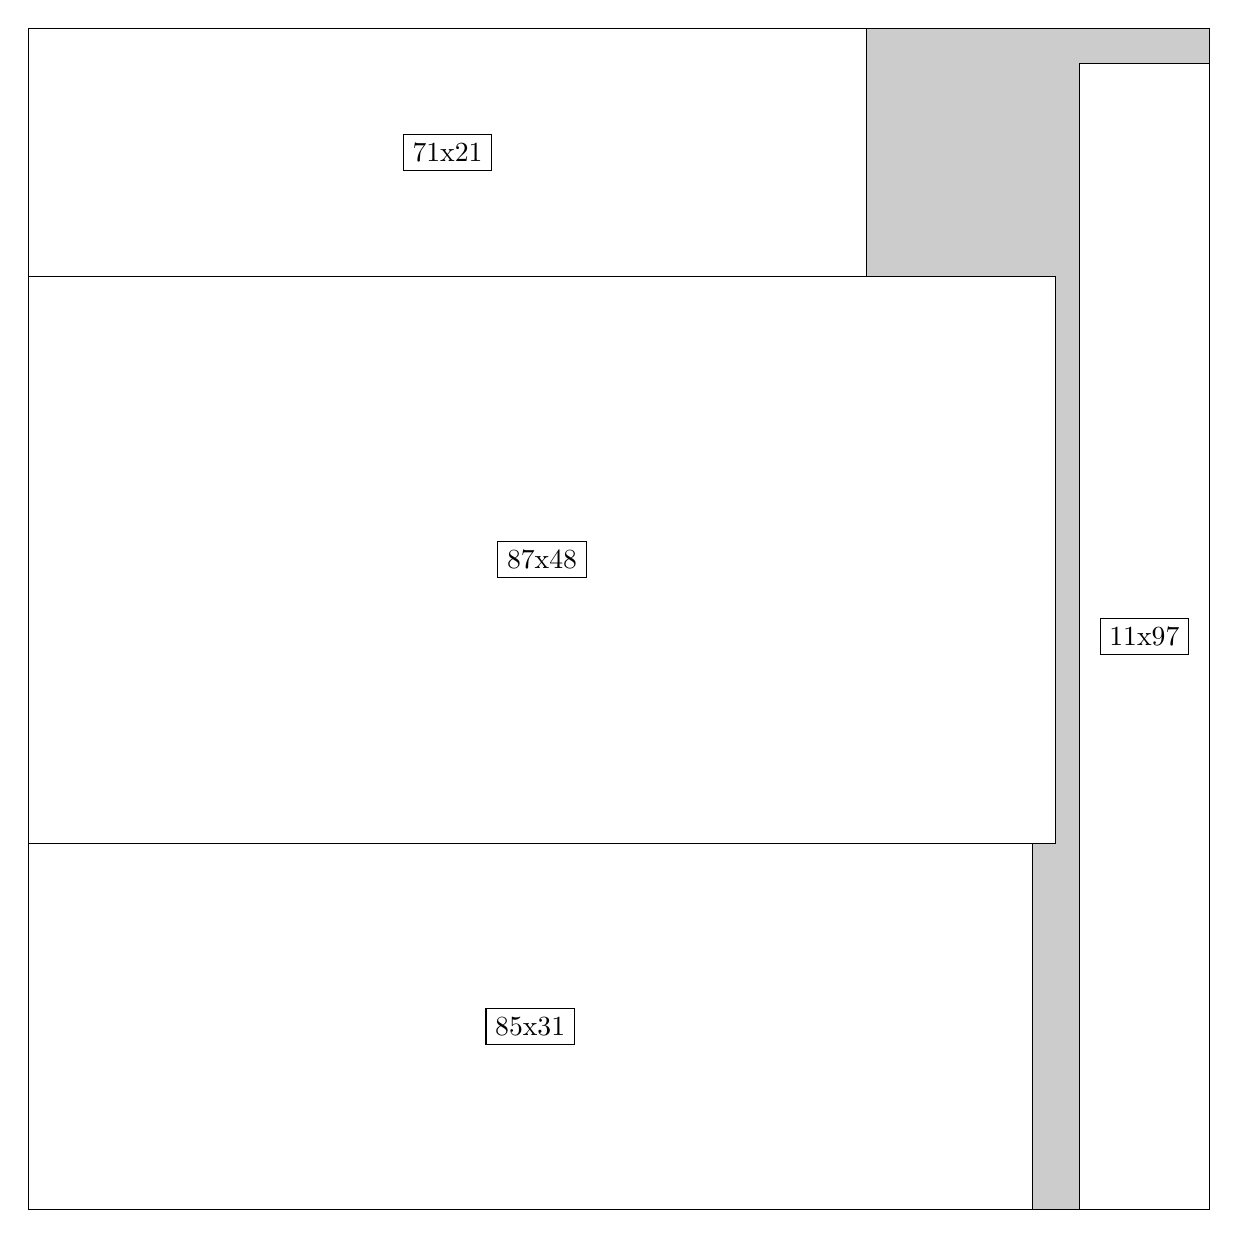
\begin{tikzpicture}[shorten >=1pt,scale=1.0,every node/.style={scale=1.0},->]
\tikzstyle{vertex}=[circle,fill=black!25,minimum size=14pt,inner sep=0pt]
\filldraw[fill=gray!40!white, draw=black] (0,0) rectangle (15.0,15.0);
\foreach \name/\x/\y/\w/\h in {85x31/0.0/0.0/12.75/4.6499999999999995,87x48/0.0/4.6499999999999995/13.049999999999999/7.199999999999999,71x21/0.0/11.85/10.65/3.15,11x97/13.35/0.0/1.65/14.549999999999999}
\filldraw[fill=white!40!white, draw=black] (\x,\y) rectangle node[draw] (\name) {\name} ++(\w,\h);
\end{tikzpicture}


w =85 , h =31 , x =0 , y =0 , v =2635
\par
w =87 , h =48 , x =0 , y =31 , v =4176
\par
w =71 , h =21 , x =0 , y =79 , v =1491
\par
w =11 , h =97 , x =89 , y =0 , v =1067
\par
\newpage


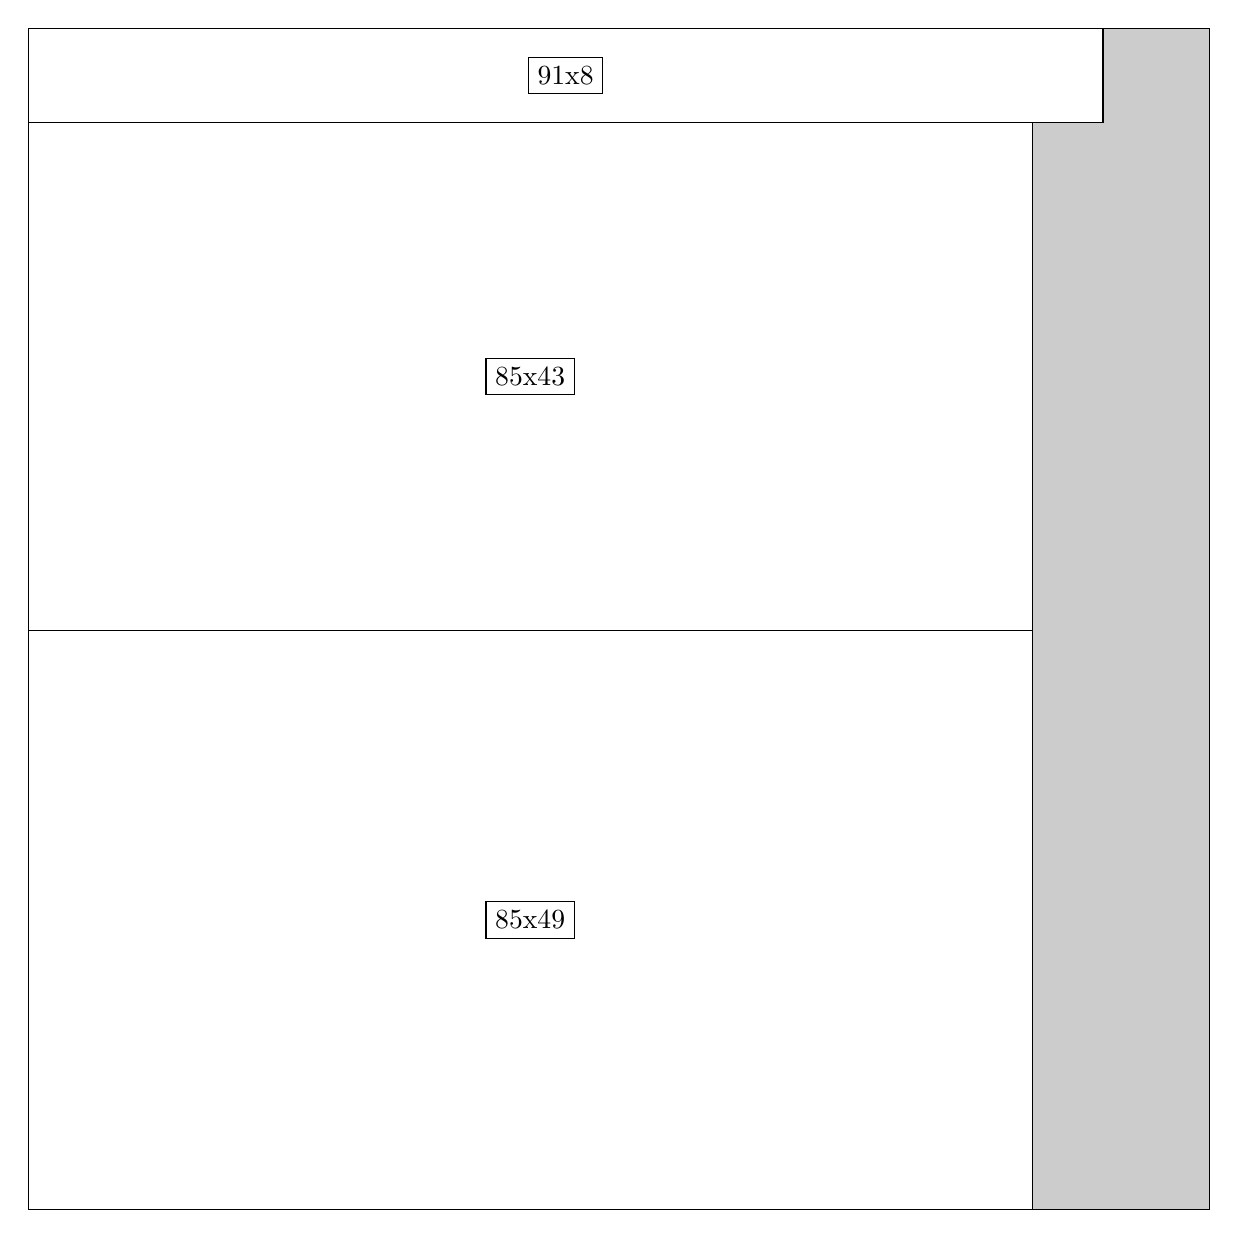
\begin{tikzpicture}[shorten >=1pt,scale=1.0,every node/.style={scale=1.0},->]
\tikzstyle{vertex}=[circle,fill=black!25,minimum size=14pt,inner sep=0pt]
\filldraw[fill=gray!40!white, draw=black] (0,0) rectangle (15.0,15.0);
\foreach \name/\x/\y/\w/\h in {85x49/0.0/0.0/12.75/7.35,85x43/0.0/7.35/12.75/6.45,91x8/0.0/13.799999999999999/13.65/1.2}
\filldraw[fill=white!40!white, draw=black] (\x,\y) rectangle node[draw] (\name) {\name} ++(\w,\h);
\end{tikzpicture}


w =85 , h =49 , x =0 , y =0 , v =4165
\par
w =85 , h =43 , x =0 , y =49 , v =3655
\par
w =91 , h =8 , x =0 , y =92 , v =728
\par
\newpage


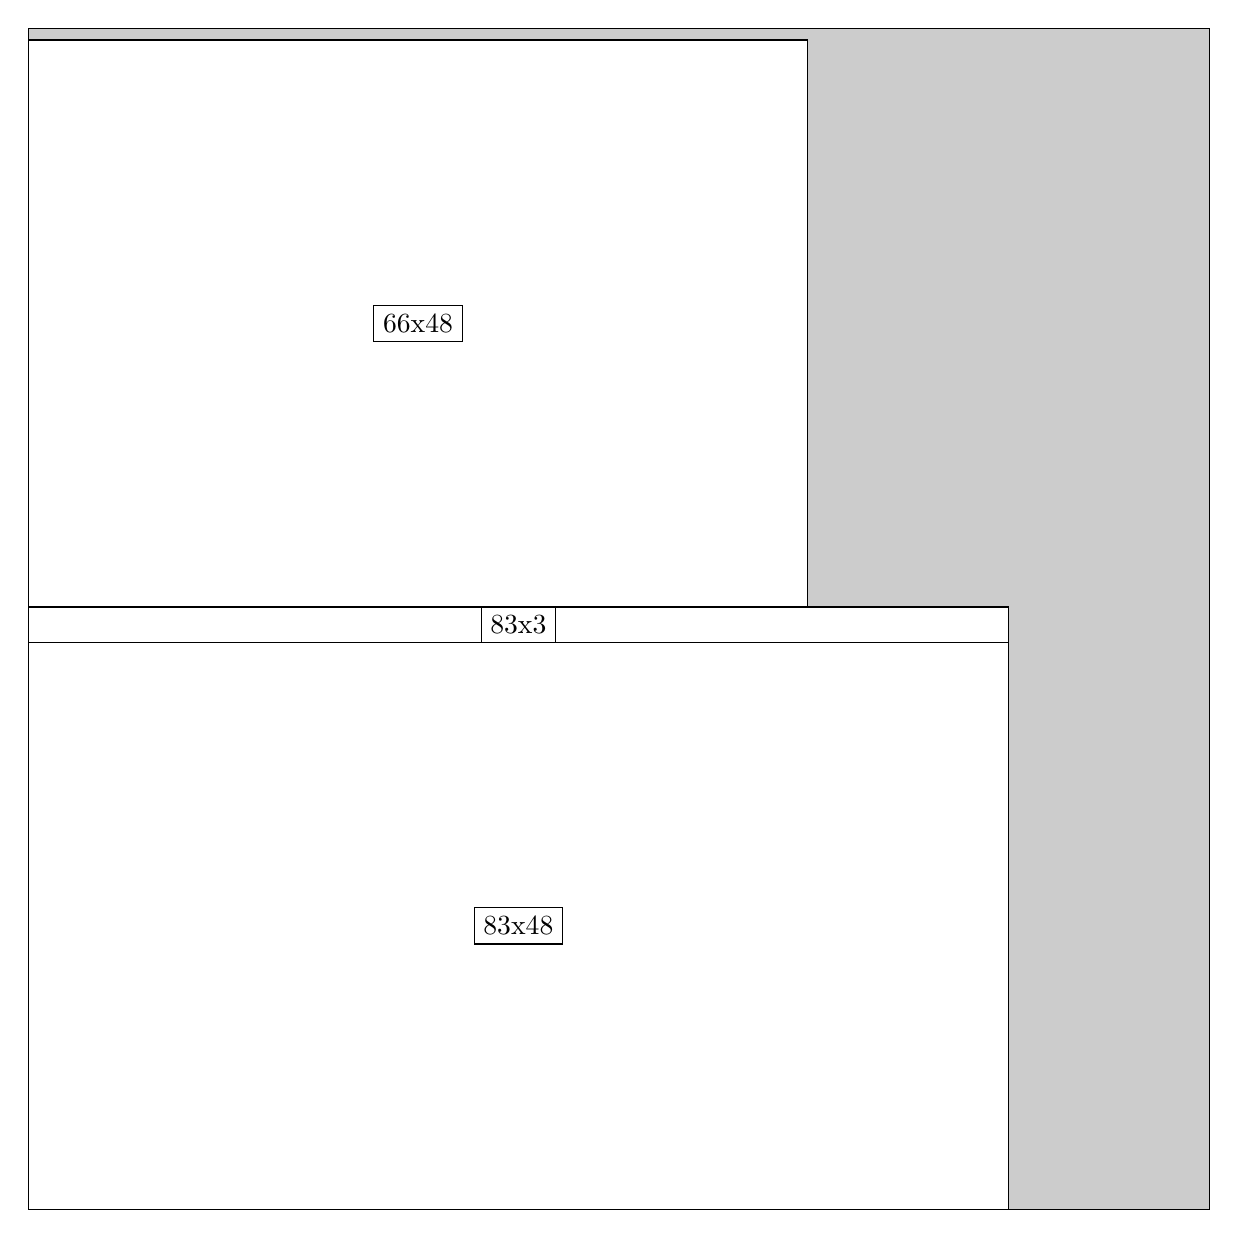
\begin{tikzpicture}[shorten >=1pt,scale=1.0,every node/.style={scale=1.0},->]
\tikzstyle{vertex}=[circle,fill=black!25,minimum size=14pt,inner sep=0pt]
\filldraw[fill=gray!40!white, draw=black] (0,0) rectangle (15.0,15.0);
\foreach \name/\x/\y/\w/\h in {83x48/0.0/0.0/12.45/7.199999999999999,66x48/0.0/7.6499999999999995/9.9/7.199999999999999,83x3/0.0/7.199999999999999/12.45/0.44999999999999996}
\filldraw[fill=white!40!white, draw=black] (\x,\y) rectangle node[draw] (\name) {\name} ++(\w,\h);
\end{tikzpicture}


w =83 , h =48 , x =0 , y =0 , v =3984
\par
w =66 , h =48 , x =0 , y =51 , v =3168
\par
w =83 , h =3 , x =0 , y =48 , v =249
\par
\newpage


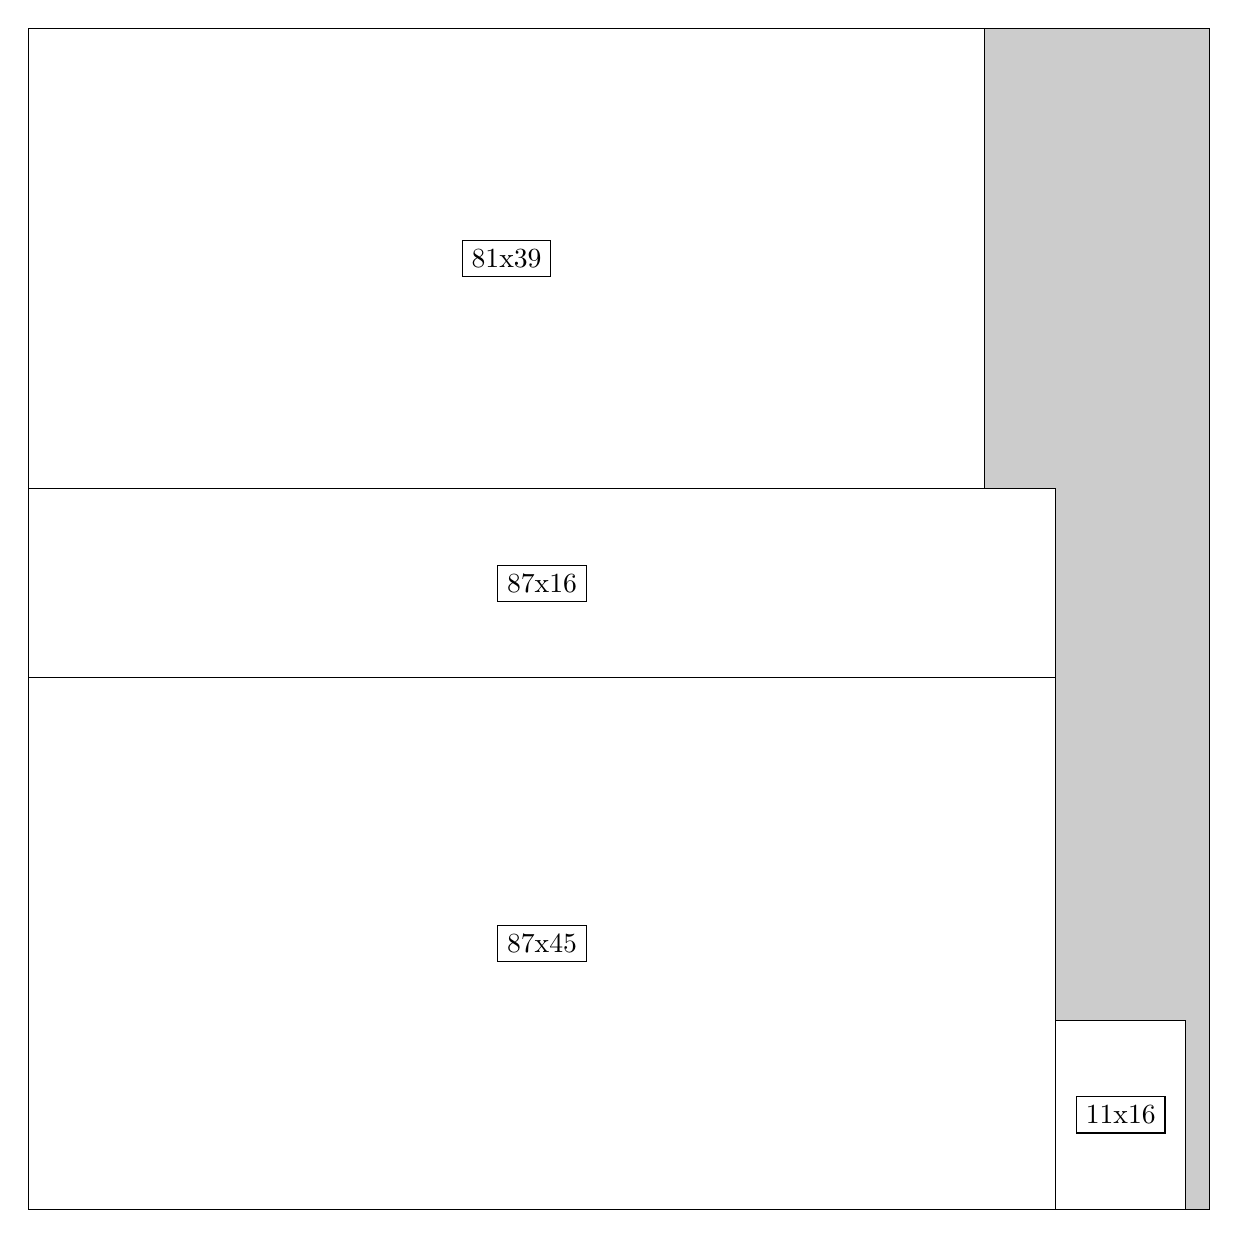
\begin{tikzpicture}[shorten >=1pt,scale=1.0,every node/.style={scale=1.0},->]
\tikzstyle{vertex}=[circle,fill=black!25,minimum size=14pt,inner sep=0pt]
\filldraw[fill=gray!40!white, draw=black] (0,0) rectangle (15.0,15.0);
\foreach \name/\x/\y/\w/\h in {87x45/0.0/0.0/13.049999999999999/6.75,81x39/0.0/9.15/12.15/5.85,87x16/0.0/6.75/13.049999999999999/2.4,11x16/13.049999999999999/0.0/1.65/2.4}
\filldraw[fill=white!40!white, draw=black] (\x,\y) rectangle node[draw] (\name) {\name} ++(\w,\h);
\end{tikzpicture}


w =87 , h =45 , x =0 , y =0 , v =3915
\par
w =81 , h =39 , x =0 , y =61 , v =3159
\par
w =87 , h =16 , x =0 , y =45 , v =1392
\par
w =11 , h =16 , x =87 , y =0 , v =176
\par
\newpage


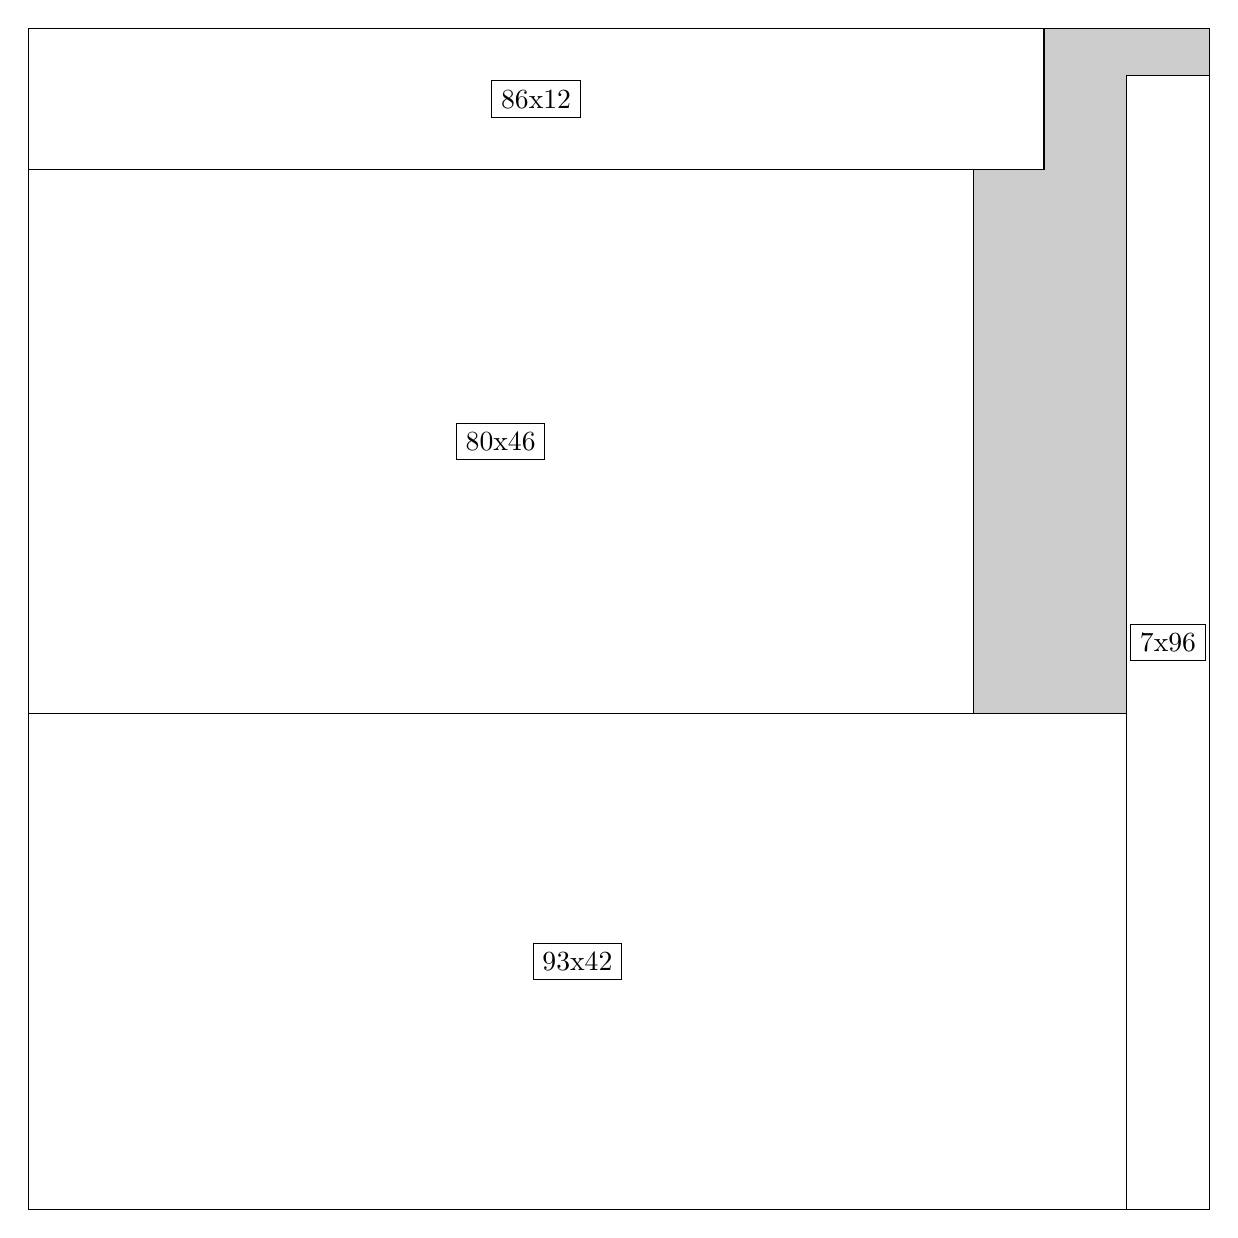
\begin{tikzpicture}[shorten >=1pt,scale=1.0,every node/.style={scale=1.0},->]
\tikzstyle{vertex}=[circle,fill=black!25,minimum size=14pt,inner sep=0pt]
\filldraw[fill=gray!40!white, draw=black] (0,0) rectangle (15.0,15.0);
\foreach \name/\x/\y/\w/\h in {93x42/0.0/0.0/13.95/6.3,80x46/0.0/6.3/12.0/6.8999999999999995,86x12/0.0/13.2/12.9/1.7999999999999998,7x96/13.95/0.0/1.05/14.399999999999999}
\filldraw[fill=white!40!white, draw=black] (\x,\y) rectangle node[draw] (\name) {\name} ++(\w,\h);
\end{tikzpicture}


w =93 , h =42 , x =0 , y =0 , v =3906
\par
w =80 , h =46 , x =0 , y =42 , v =3680
\par
w =86 , h =12 , x =0 , y =88 , v =1032
\par
w =7 , h =96 , x =93 , y =0 , v =672
\par
\newpage


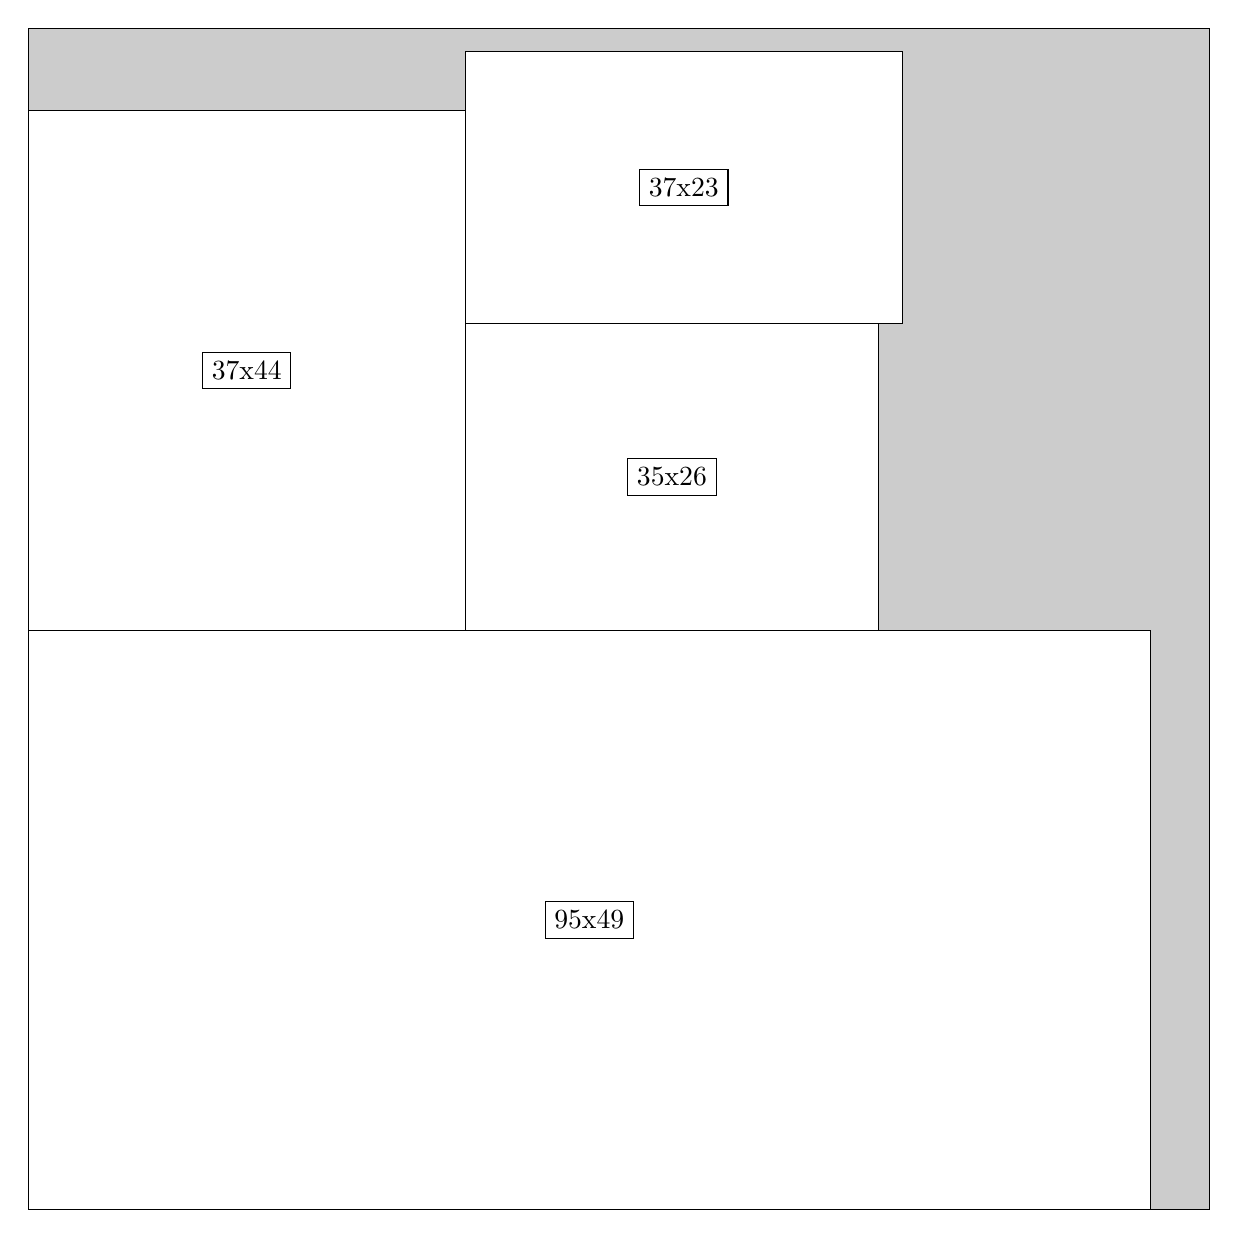
\begin{tikzpicture}[shorten >=1pt,scale=1.0,every node/.style={scale=1.0},->]
\tikzstyle{vertex}=[circle,fill=black!25,minimum size=14pt,inner sep=0pt]
\filldraw[fill=gray!40!white, draw=black] (0,0) rectangle (15.0,15.0);
\foreach \name/\x/\y/\w/\h in {95x49/0.0/0.0/14.25/7.35,37x44/0.0/7.35/5.55/6.6,35x26/5.55/7.35/5.25/3.9,37x23/5.55/11.25/5.55/3.4499999999999997}
\filldraw[fill=white!40!white, draw=black] (\x,\y) rectangle node[draw] (\name) {\name} ++(\w,\h);
\end{tikzpicture}


w =95 , h =49 , x =0 , y =0 , v =4655
\par
w =37 , h =44 , x =0 , y =49 , v =1628
\par
w =35 , h =26 , x =37 , y =49 , v =910
\par
w =37 , h =23 , x =37 , y =75 , v =851
\par
\newpage


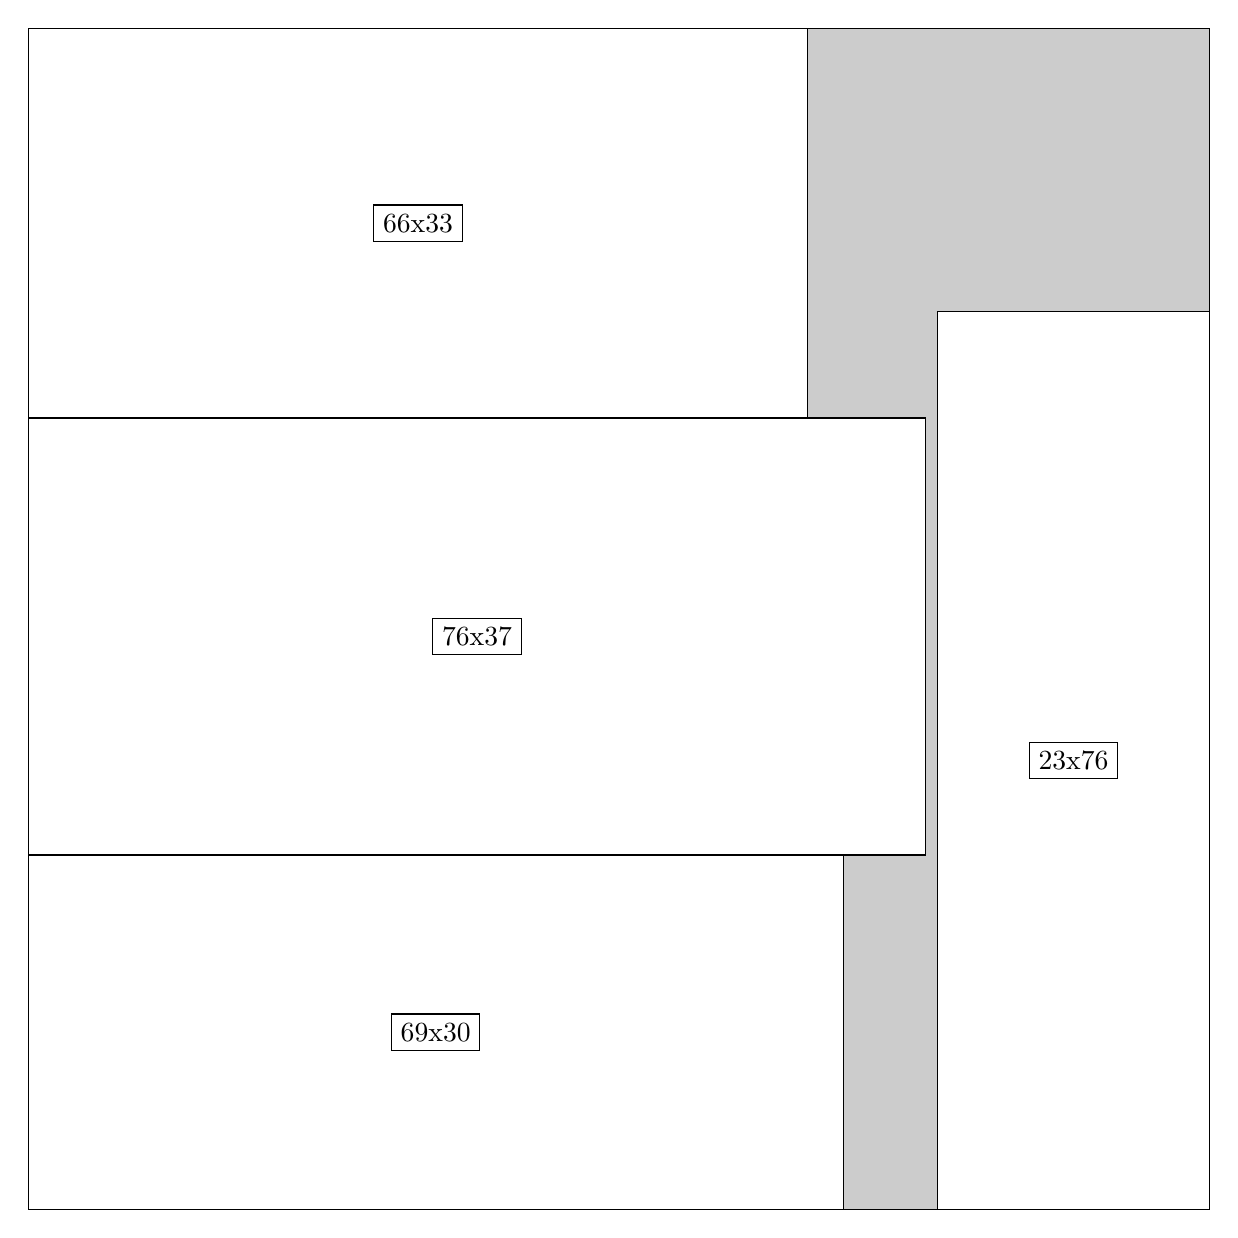
\begin{tikzpicture}[shorten >=1pt,scale=1.0,every node/.style={scale=1.0},->]
\tikzstyle{vertex}=[circle,fill=black!25,minimum size=14pt,inner sep=0pt]
\filldraw[fill=gray!40!white, draw=black] (0,0) rectangle (15.0,15.0);
\foreach \name/\x/\y/\w/\h in {66x33/0.0/10.049999999999999/9.9/4.95,76x37/0.0/4.5/11.4/5.55,69x30/0.0/0.0/10.35/4.5,23x76/11.549999999999999/0.0/3.4499999999999997/11.4}
\filldraw[fill=white!40!white, draw=black] (\x,\y) rectangle node[draw] (\name) {\name} ++(\w,\h);
\end{tikzpicture}


w =66 , h =33 , x =0 , y =67 , v =2178
\par
w =76 , h =37 , x =0 , y =30 , v =2812
\par
w =69 , h =30 , x =0 , y =0 , v =2070
\par
w =23 , h =76 , x =77 , y =0 , v =1748
\par
\newpage


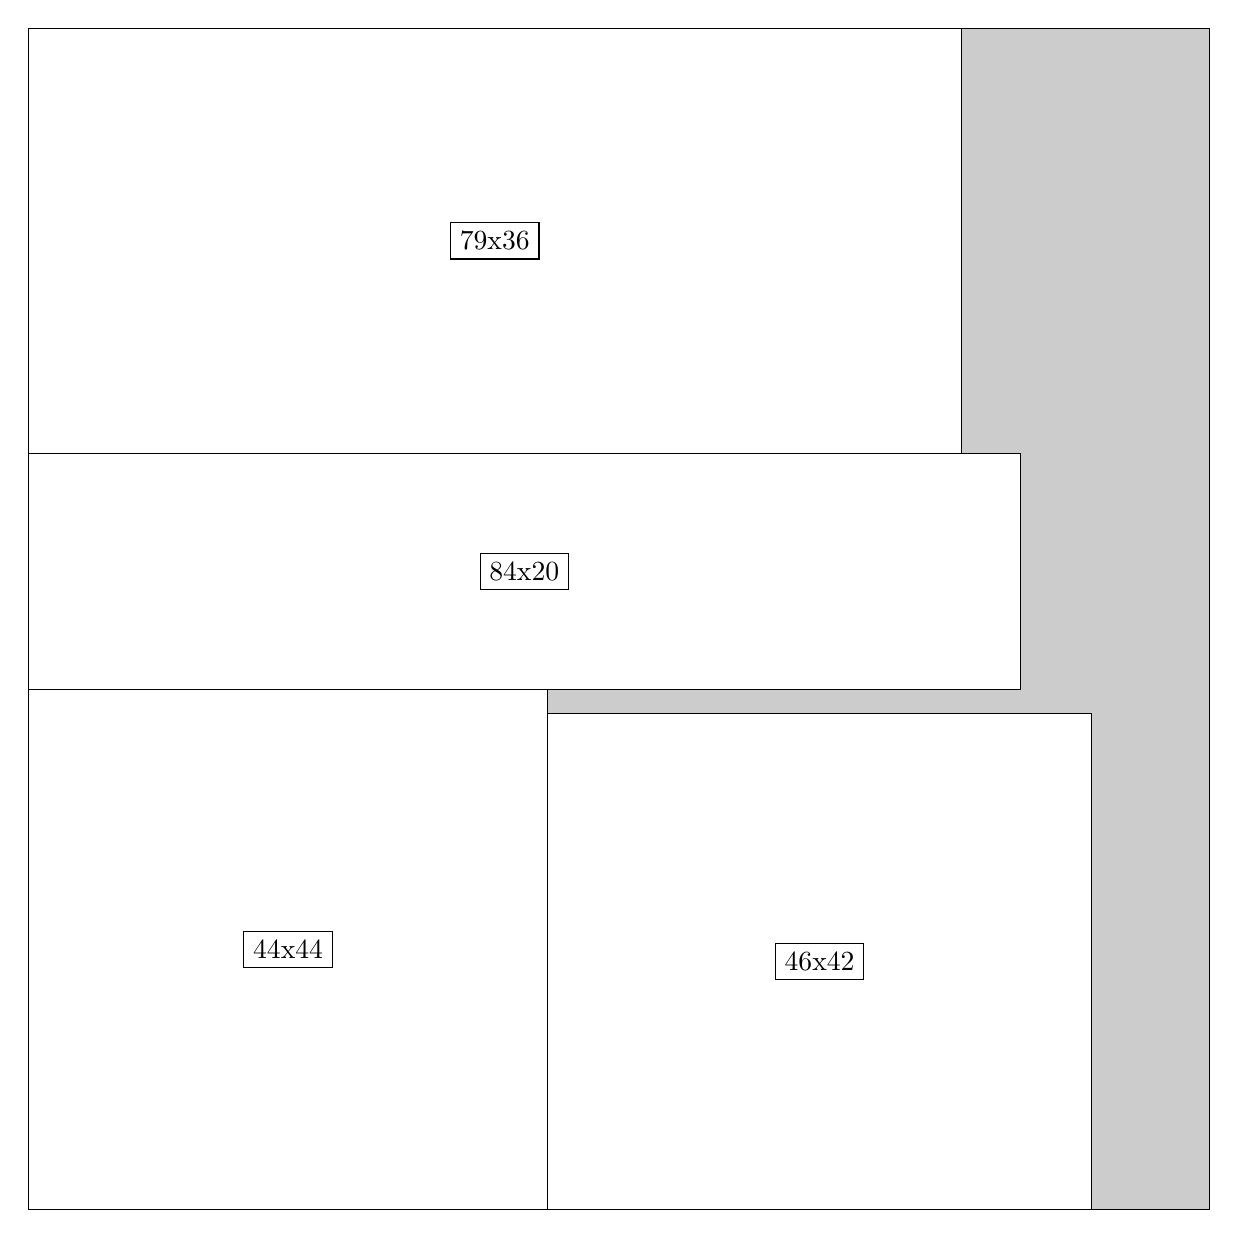
\begin{tikzpicture}[shorten >=1pt,scale=1.0,every node/.style={scale=1.0},->]
\tikzstyle{vertex}=[circle,fill=black!25,minimum size=14pt,inner sep=0pt]
\filldraw[fill=gray!40!white, draw=black] (0,0) rectangle (15.0,15.0);
\foreach \name/\x/\y/\w/\h in {79x36/0.0/9.6/11.85/5.3999999999999995,44x44/0.0/0.0/6.6/6.6,46x42/6.6/0.0/6.8999999999999995/6.3,84x20/0.0/6.6/12.6/3.0}
\filldraw[fill=white!40!white, draw=black] (\x,\y) rectangle node[draw] (\name) {\name} ++(\w,\h);
\end{tikzpicture}


w =79 , h =36 , x =0 , y =64 , v =2844
\par
w =44 , h =44 , x =0 , y =0 , v =1936
\par
w =46 , h =42 , x =44 , y =0 , v =1932
\par
w =84 , h =20 , x =0 , y =44 , v =1680
\par
\newpage


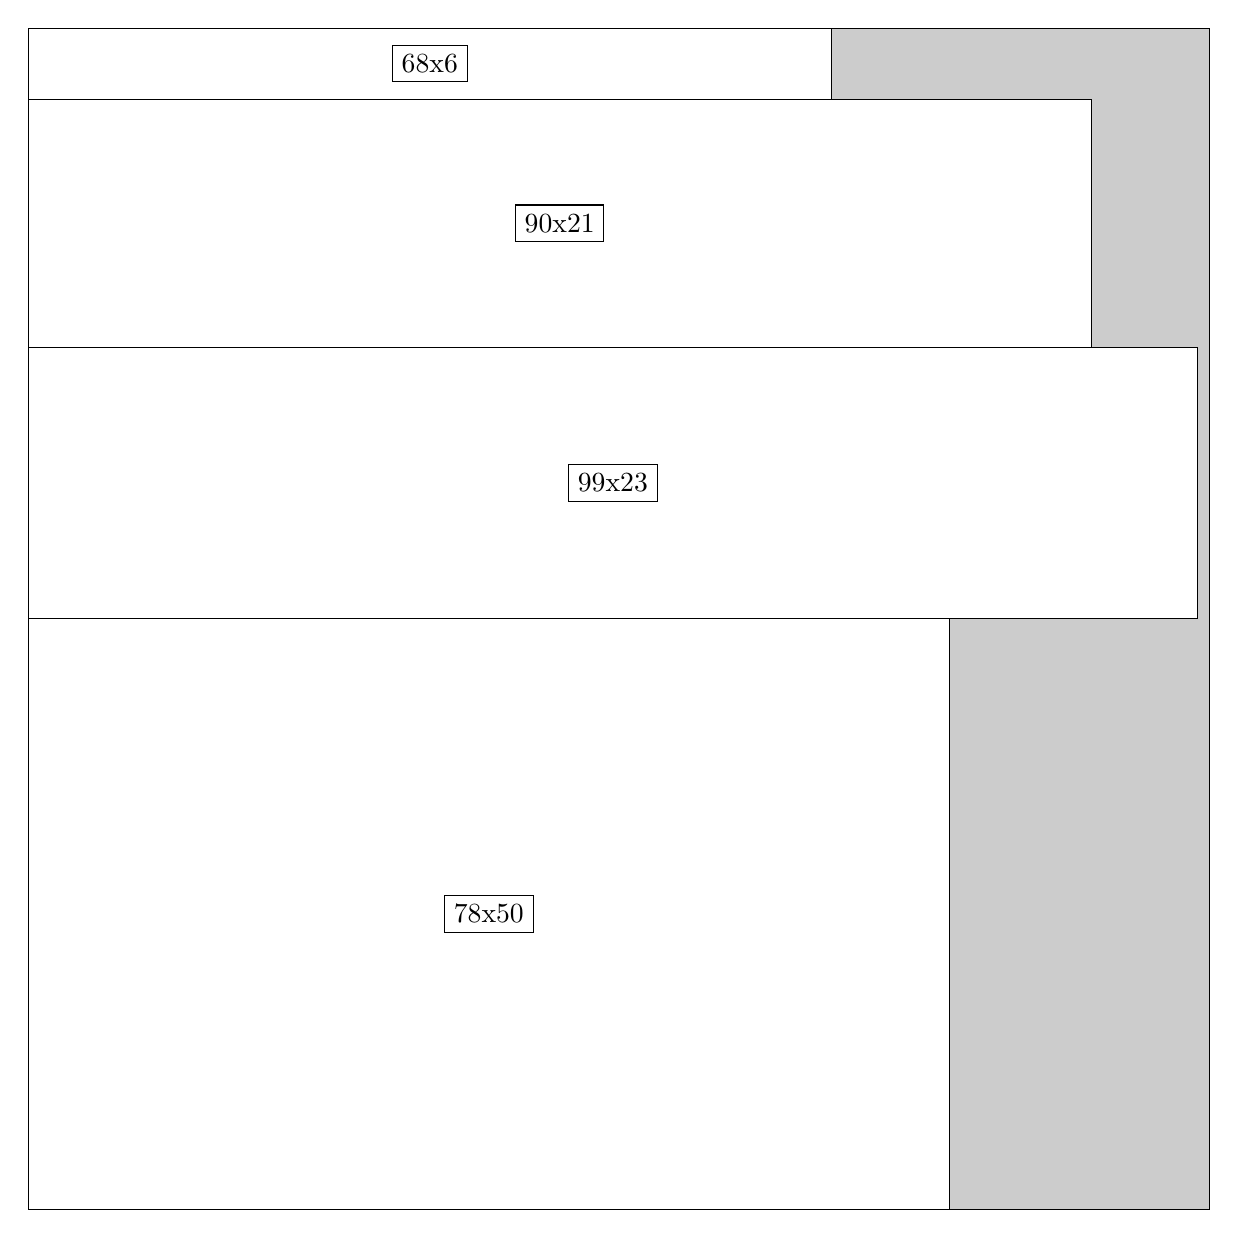
\begin{tikzpicture}[shorten >=1pt,scale=1.0,every node/.style={scale=1.0},->]
\tikzstyle{vertex}=[circle,fill=black!25,minimum size=14pt,inner sep=0pt]
\filldraw[fill=gray!40!white, draw=black] (0,0) rectangle (15.0,15.0);
\foreach \name/\x/\y/\w/\h in {78x50/0.0/0.0/11.7/7.5,99x23/0.0/7.5/14.85/3.4499999999999997,90x21/0.0/10.95/13.5/3.15,68x6/0.0/14.1/10.2/0.8999999999999999}
\filldraw[fill=white!40!white, draw=black] (\x,\y) rectangle node[draw] (\name) {\name} ++(\w,\h);
\end{tikzpicture}


w =78 , h =50 , x =0 , y =0 , v =3900
\par
w =99 , h =23 , x =0 , y =50 , v =2277
\par
w =90 , h =21 , x =0 , y =73 , v =1890
\par
w =68 , h =6 , x =0 , y =94 , v =408
\par
\newpage


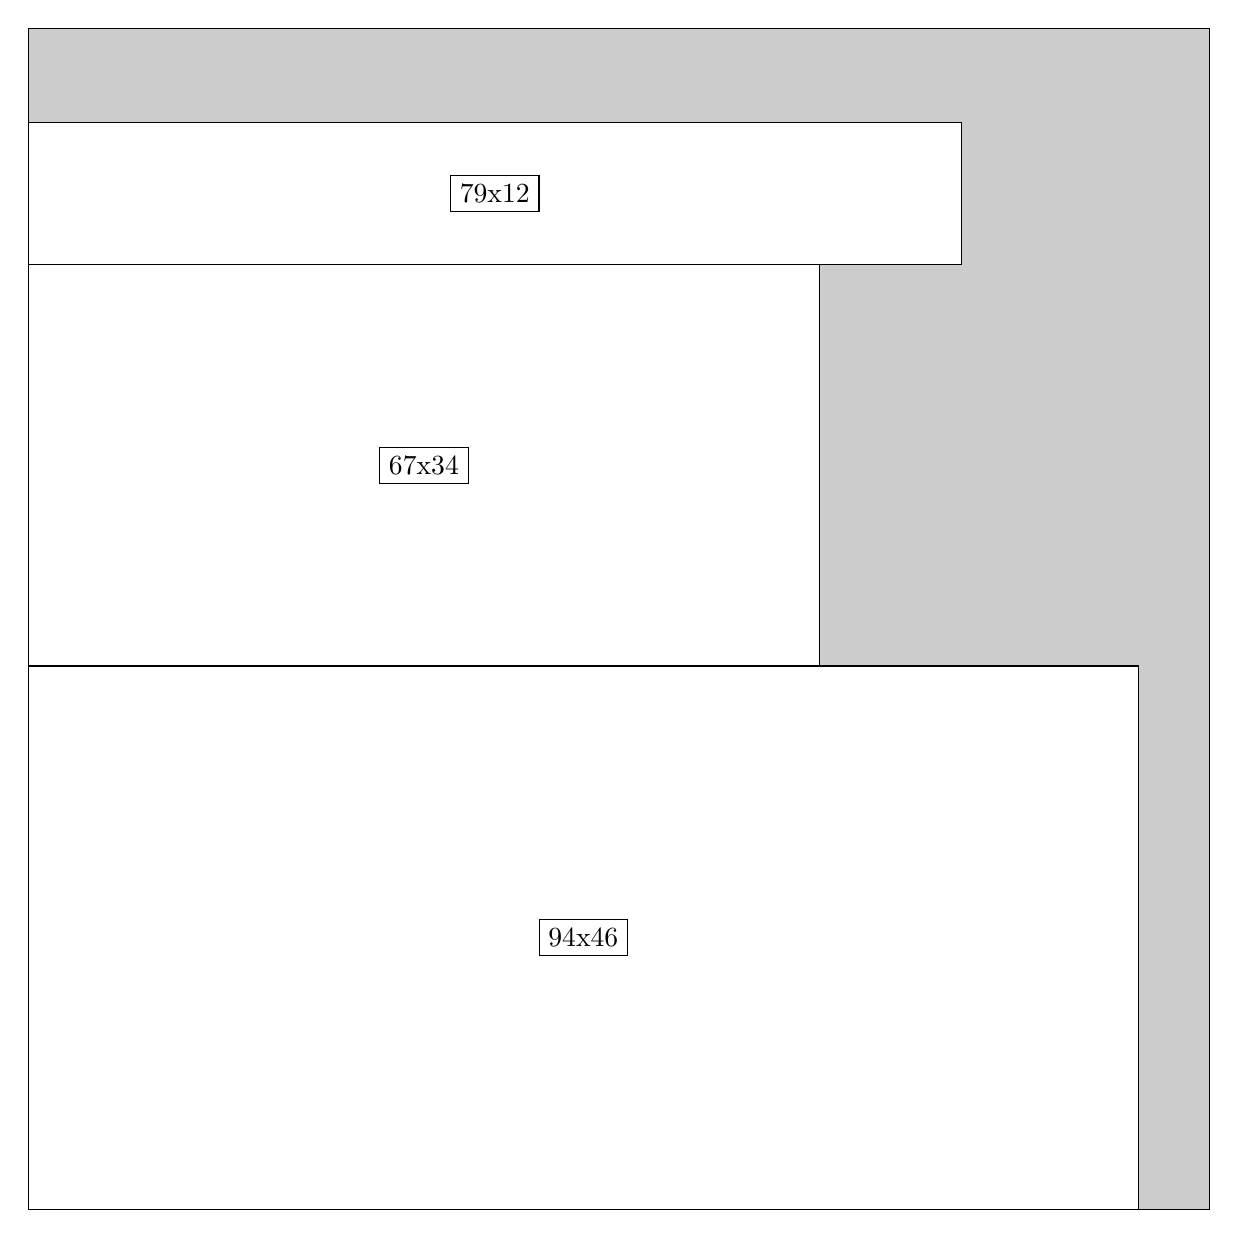
\begin{tikzpicture}[shorten >=1pt,scale=1.0,every node/.style={scale=1.0},->]
\tikzstyle{vertex}=[circle,fill=black!25,minimum size=14pt,inner sep=0pt]
\filldraw[fill=gray!40!white, draw=black] (0,0) rectangle (15.0,15.0);
\foreach \name/\x/\y/\w/\h in {94x46/0.0/0.0/14.1/6.8999999999999995,67x34/0.0/6.8999999999999995/10.049999999999999/5.1,79x12/0.0/12.0/11.85/1.7999999999999998}
\filldraw[fill=white!40!white, draw=black] (\x,\y) rectangle node[draw] (\name) {\name} ++(\w,\h);
\end{tikzpicture}


w =94 , h =46 , x =0 , y =0 , v =4324
\par
w =67 , h =34 , x =0 , y =46 , v =2278
\par
w =79 , h =12 , x =0 , y =80 , v =948
\par
\newpage


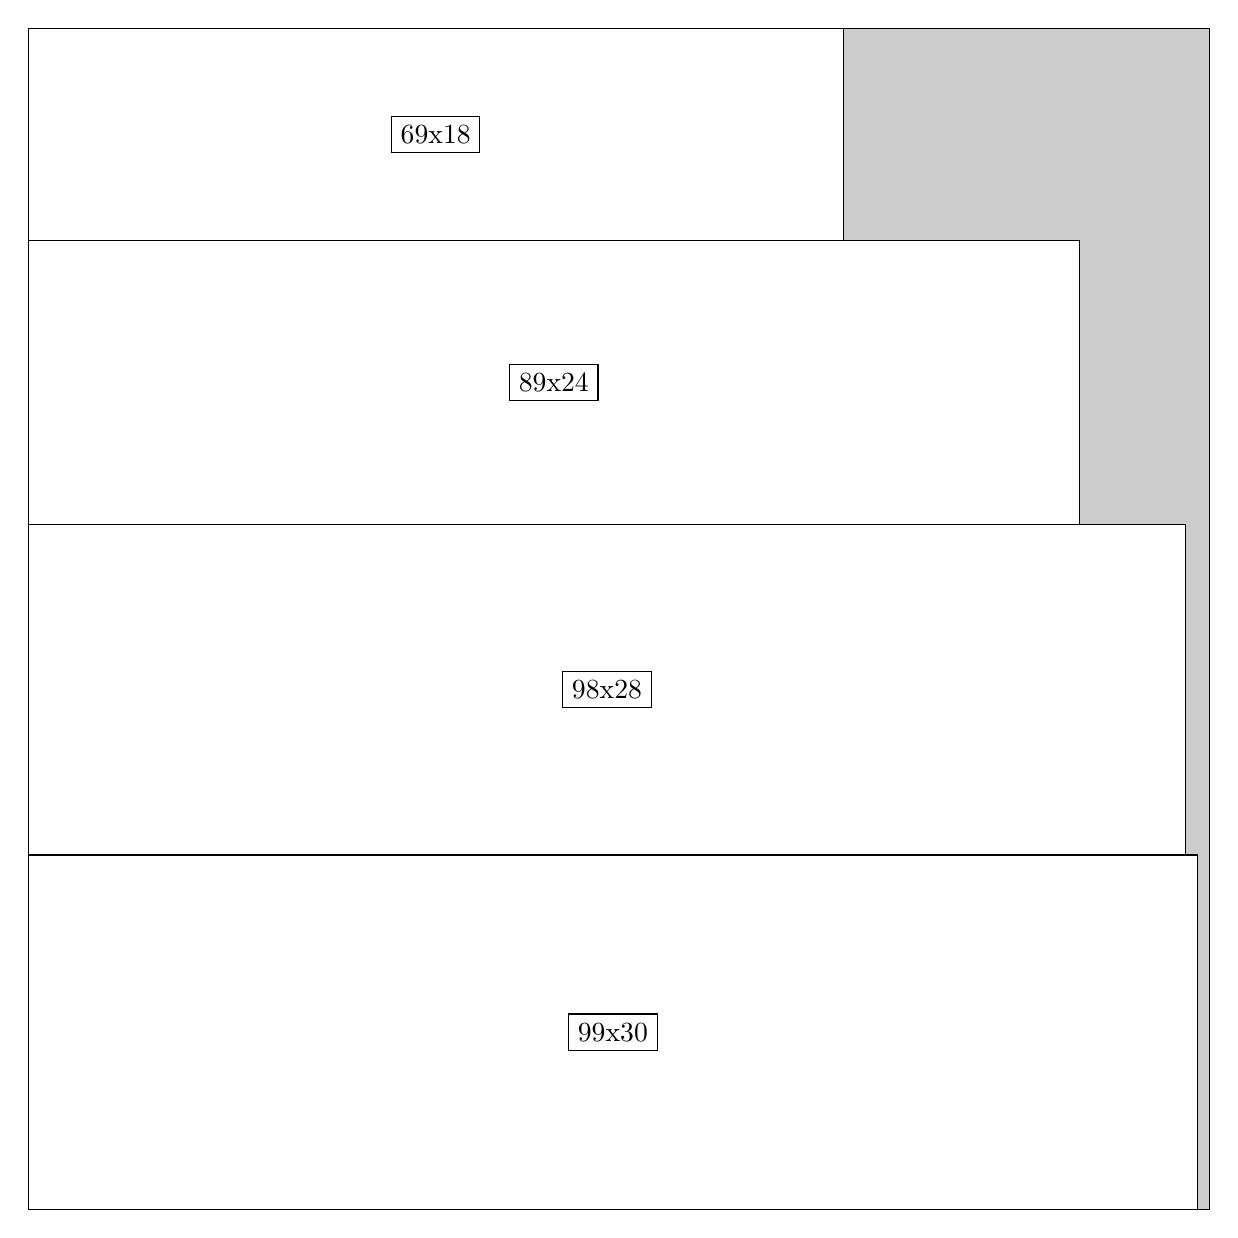
\begin{tikzpicture}[shorten >=1pt,scale=1.0,every node/.style={scale=1.0},->]
\tikzstyle{vertex}=[circle,fill=black!25,minimum size=14pt,inner sep=0pt]
\filldraw[fill=gray!40!white, draw=black] (0,0) rectangle (15.0,15.0);
\foreach \name/\x/\y/\w/\h in {99x30/0.0/0.0/14.85/4.5,98x28/0.0/4.5/14.7/4.2,89x24/0.0/8.7/13.35/3.5999999999999996,69x18/0.0/12.299999999999999/10.35/2.6999999999999997}
\filldraw[fill=white!40!white, draw=black] (\x,\y) rectangle node[draw] (\name) {\name} ++(\w,\h);
\end{tikzpicture}


w =99 , h =30 , x =0 , y =0 , v =2970
\par
w =98 , h =28 , x =0 , y =30 , v =2744
\par
w =89 , h =24 , x =0 , y =58 , v =2136
\par
w =69 , h =18 , x =0 , y =82 , v =1242
\par
\newpage


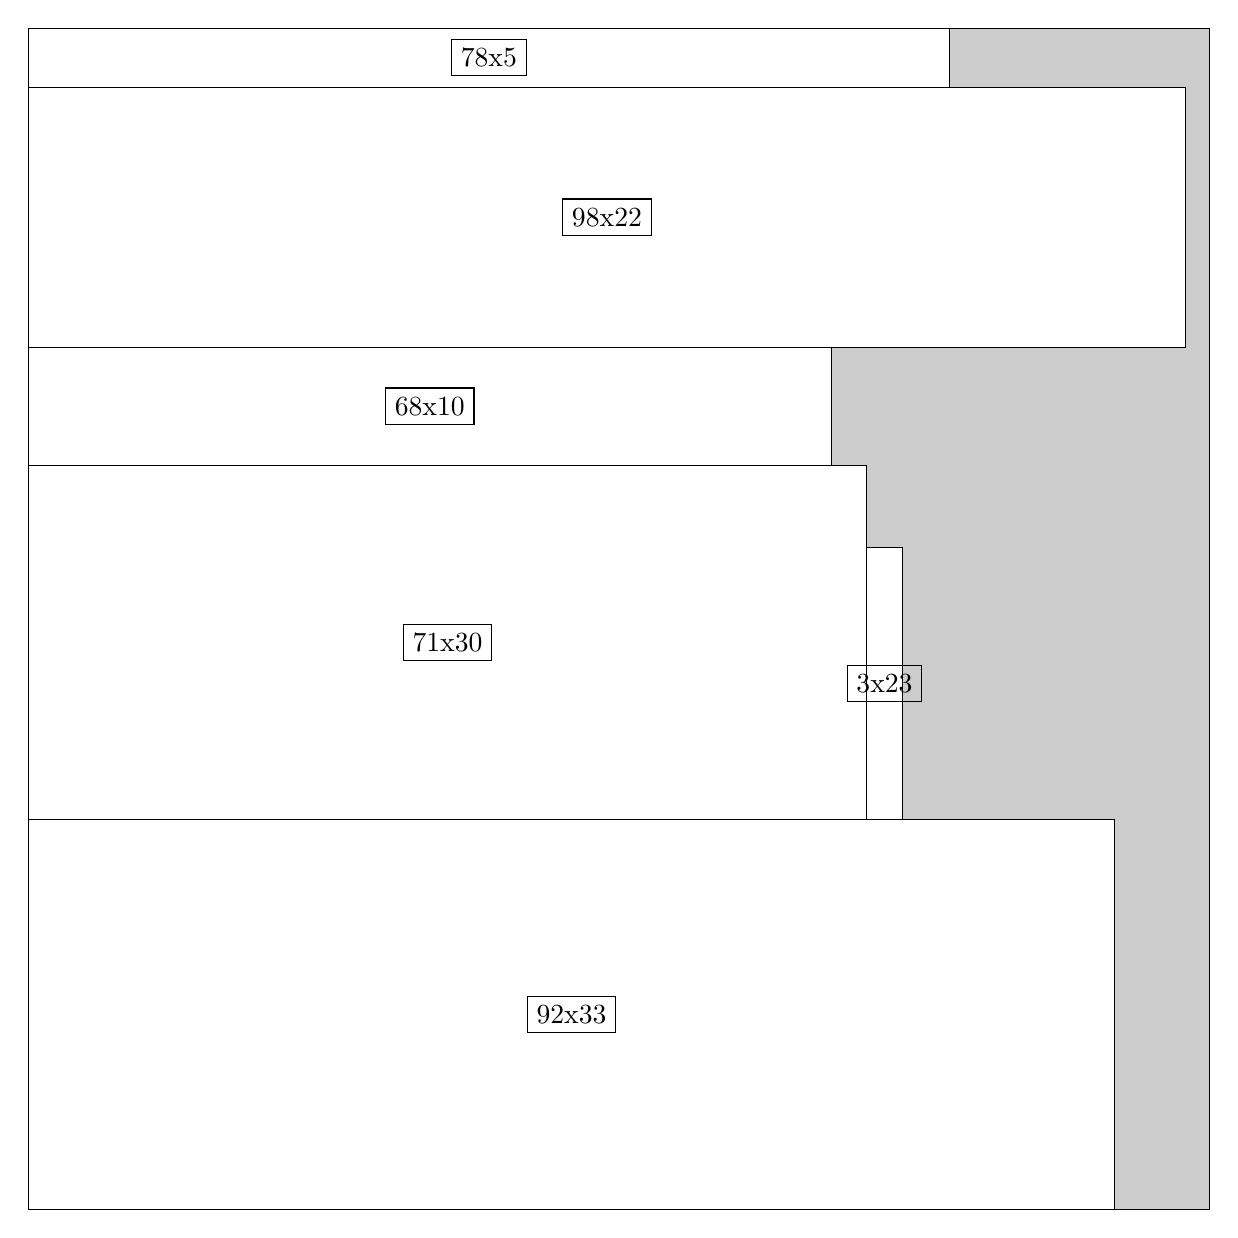
\begin{tikzpicture}[shorten >=1pt,scale=1.0,every node/.style={scale=1.0},->]
\tikzstyle{vertex}=[circle,fill=black!25,minimum size=14pt,inner sep=0pt]
\filldraw[fill=gray!40!white, draw=black] (0,0) rectangle (15.0,15.0);
\foreach \name/\x/\y/\w/\h in {92x33/0.0/0.0/13.799999999999999/4.95,98x22/0.0/10.95/14.7/3.3,71x30/0.0/4.95/10.65/4.5,68x10/0.0/9.45/10.2/1.5,78x5/0.0/14.25/11.7/0.75,3x23/10.65/4.95/0.44999999999999996/3.4499999999999997}
\filldraw[fill=white!40!white, draw=black] (\x,\y) rectangle node[draw] (\name) {\name} ++(\w,\h);
\end{tikzpicture}


w =92 , h =33 , x =0 , y =0 , v =3036
\par
w =98 , h =22 , x =0 , y =73 , v =2156
\par
w =71 , h =30 , x =0 , y =33 , v =2130
\par
w =68 , h =10 , x =0 , y =63 , v =680
\par
w =78 , h =5 , x =0 , y =95 , v =390
\par
w =3 , h =23 , x =71 , y =33 , v =69
\par
\newpage


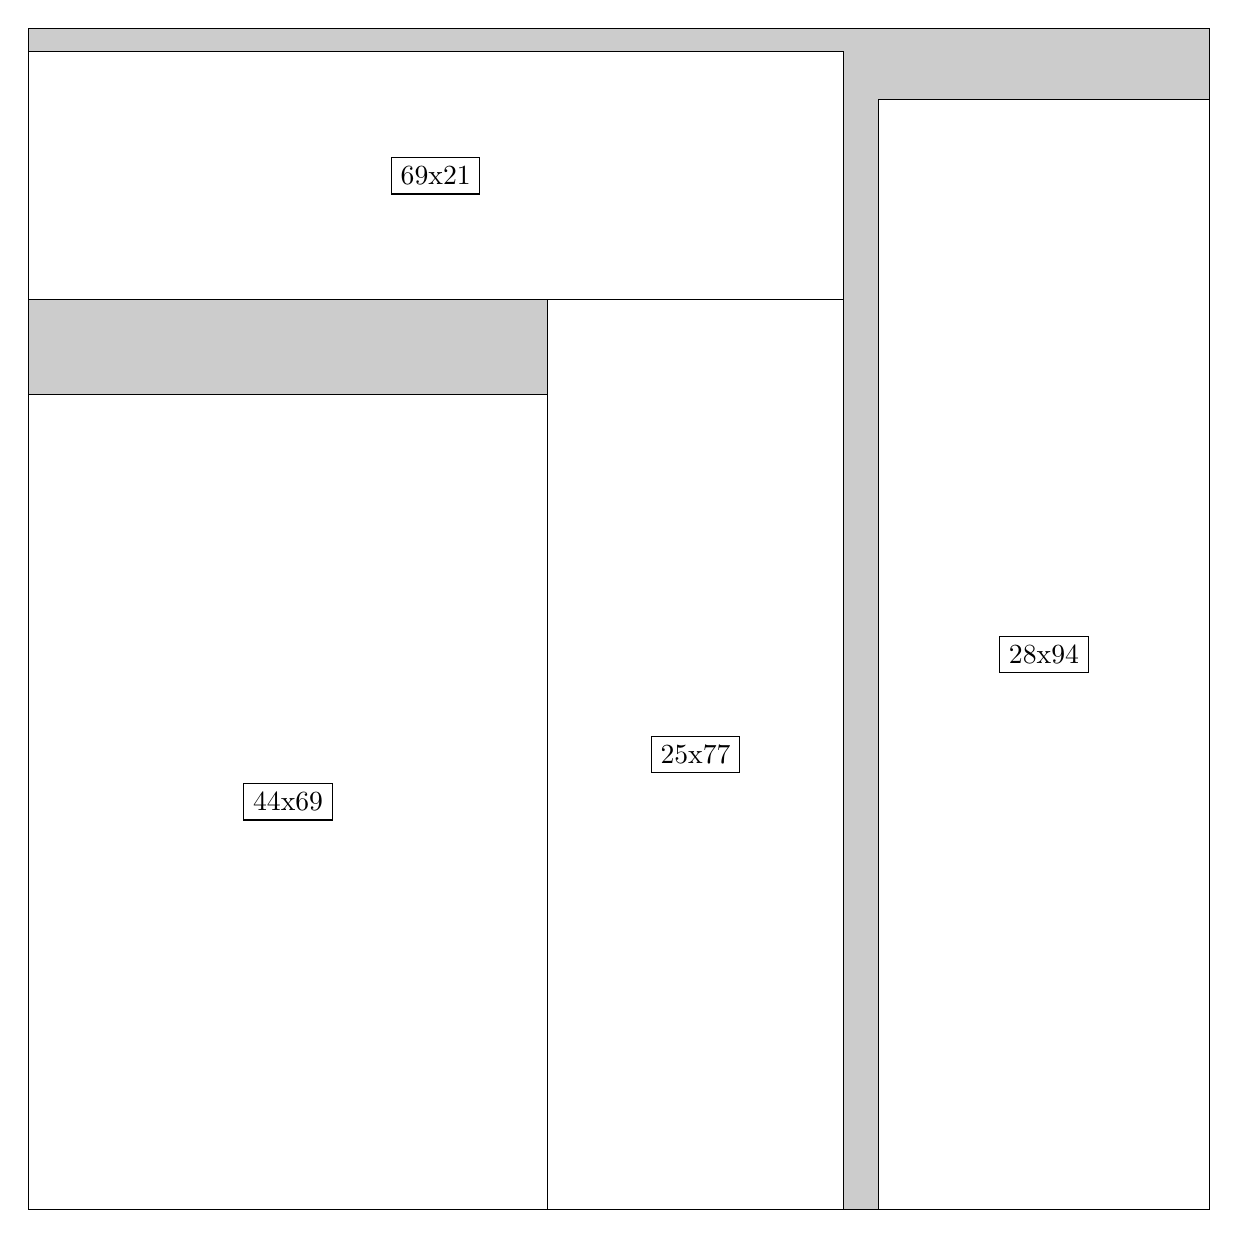
\begin{tikzpicture}[shorten >=1pt,scale=1.0,every node/.style={scale=1.0},->]
\tikzstyle{vertex}=[circle,fill=black!25,minimum size=14pt,inner sep=0pt]
\filldraw[fill=gray!40!white, draw=black] (0,0) rectangle (15.0,15.0);
\foreach \name/\x/\y/\w/\h in {44x69/0.0/0.0/6.6/10.35,28x94/10.799999999999999/0.0/4.2/14.1,25x77/6.6/0.0/3.75/11.549999999999999,69x21/0.0/11.549999999999999/10.35/3.15}
\filldraw[fill=white!40!white, draw=black] (\x,\y) rectangle node[draw] (\name) {\name} ++(\w,\h);
\end{tikzpicture}


w =44 , h =69 , x =0 , y =0 , v =3036
\par
w =28 , h =94 , x =72 , y =0 , v =2632
\par
w =25 , h =77 , x =44 , y =0 , v =1925
\par
w =69 , h =21 , x =0 , y =77 , v =1449
\par
\newpage


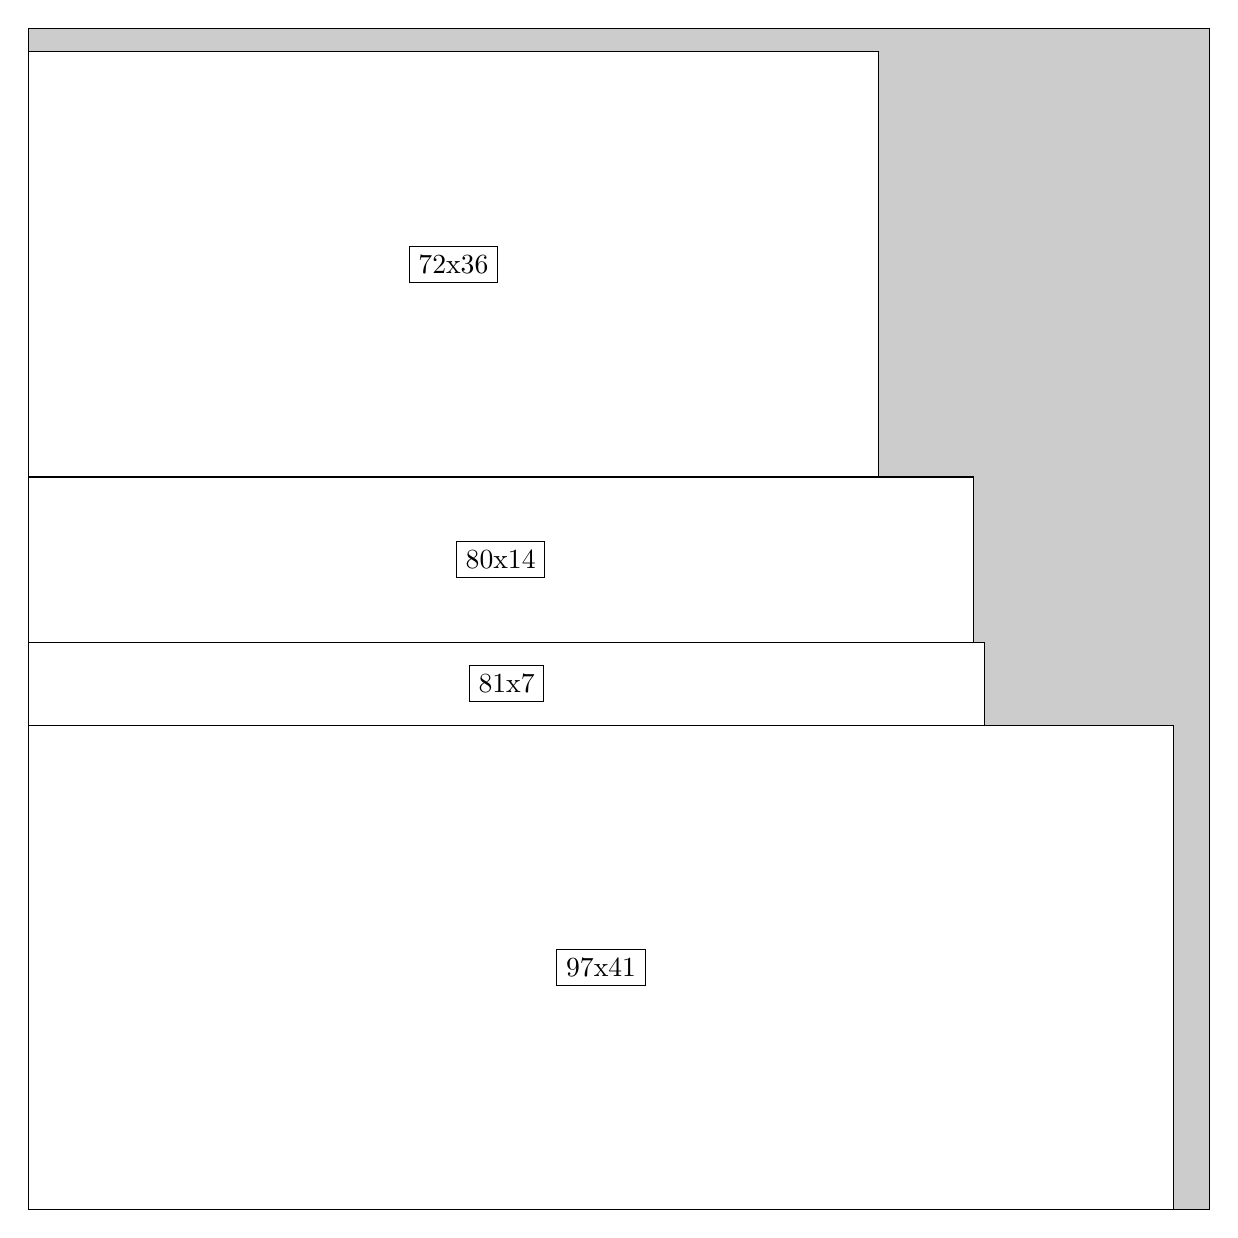
\begin{tikzpicture}[shorten >=1pt,scale=1.0,every node/.style={scale=1.0},->]
\tikzstyle{vertex}=[circle,fill=black!25,minimum size=14pt,inner sep=0pt]
\filldraw[fill=gray!40!white, draw=black] (0,0) rectangle (15.0,15.0);
\foreach \name/\x/\y/\w/\h in {97x41/0.0/0.0/14.549999999999999/6.1499999999999995,72x36/0.0/9.299999999999999/10.799999999999999/5.3999999999999995,80x14/0.0/7.199999999999999/12.0/2.1,81x7/0.0/6.1499999999999995/12.15/1.05}
\filldraw[fill=white!40!white, draw=black] (\x,\y) rectangle node[draw] (\name) {\name} ++(\w,\h);
\end{tikzpicture}


w =97 , h =41 , x =0 , y =0 , v =3977
\par
w =72 , h =36 , x =0 , y =62 , v =2592
\par
w =80 , h =14 , x =0 , y =48 , v =1120
\par
w =81 , h =7 , x =0 , y =41 , v =567
\par
\newpage


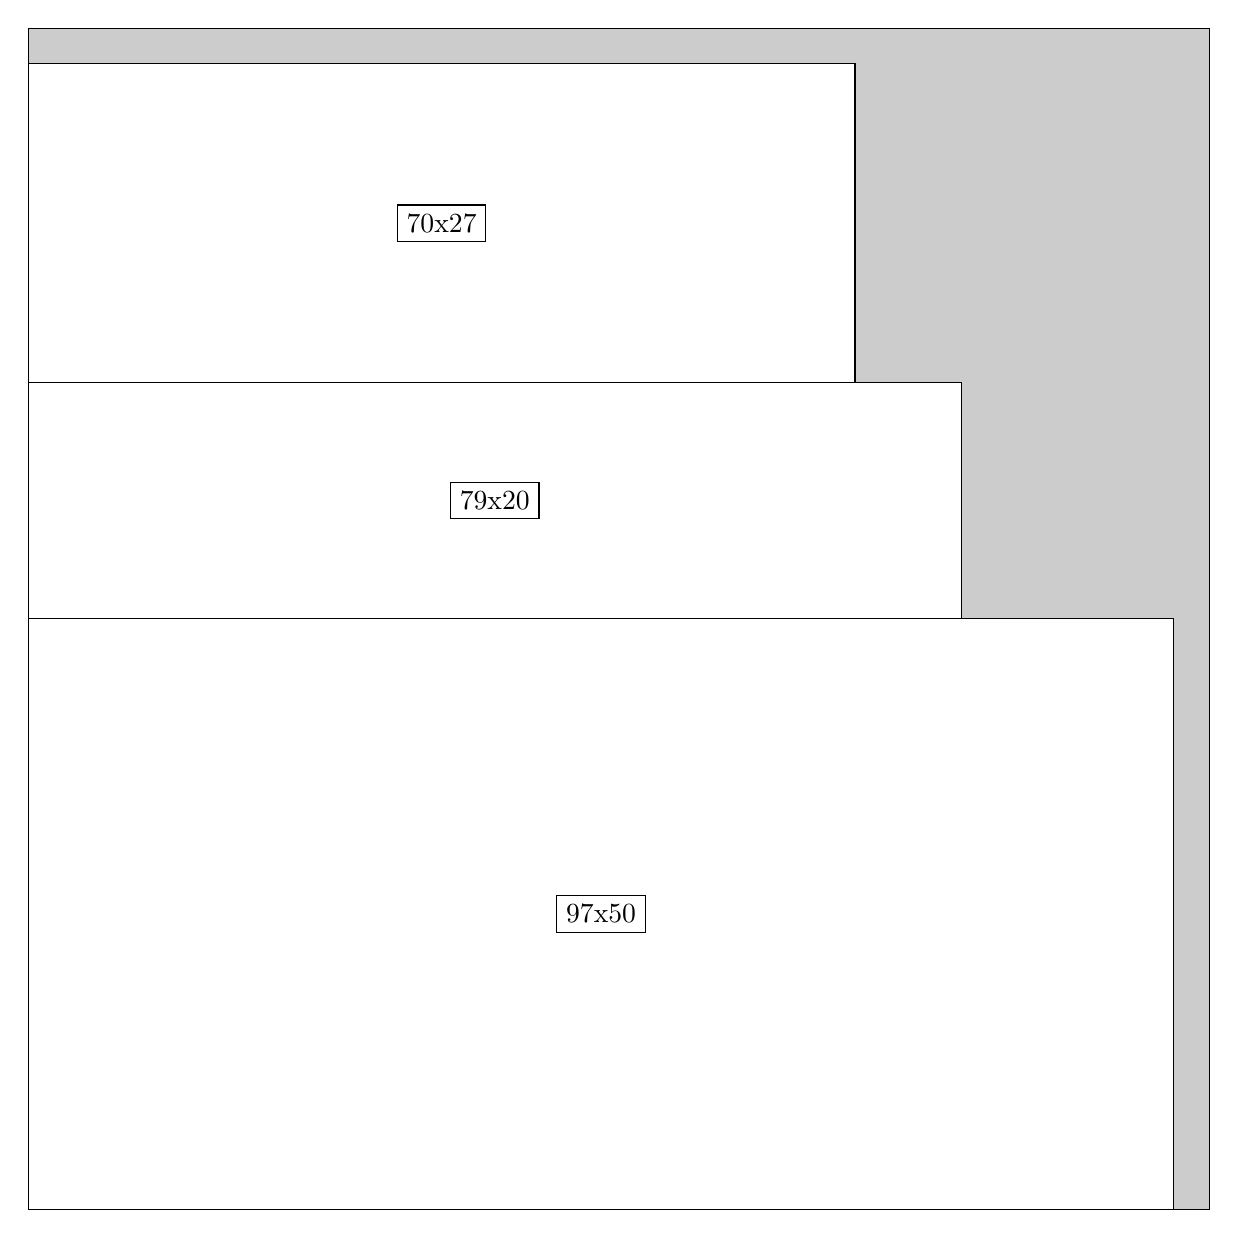
\begin{tikzpicture}[shorten >=1pt,scale=1.0,every node/.style={scale=1.0},->]
\tikzstyle{vertex}=[circle,fill=black!25,minimum size=14pt,inner sep=0pt]
\filldraw[fill=gray!40!white, draw=black] (0,0) rectangle (15.0,15.0);
\foreach \name/\x/\y/\w/\h in {97x50/0.0/0.0/14.549999999999999/7.5,70x27/0.0/10.5/10.5/4.05,79x20/0.0/7.5/11.85/3.0}
\filldraw[fill=white!40!white, draw=black] (\x,\y) rectangle node[draw] (\name) {\name} ++(\w,\h);
\end{tikzpicture}


w =97 , h =50 , x =0 , y =0 , v =4850
\par
w =70 , h =27 , x =0 , y =70 , v =1890
\par
w =79 , h =20 , x =0 , y =50 , v =1580
\par
\newpage


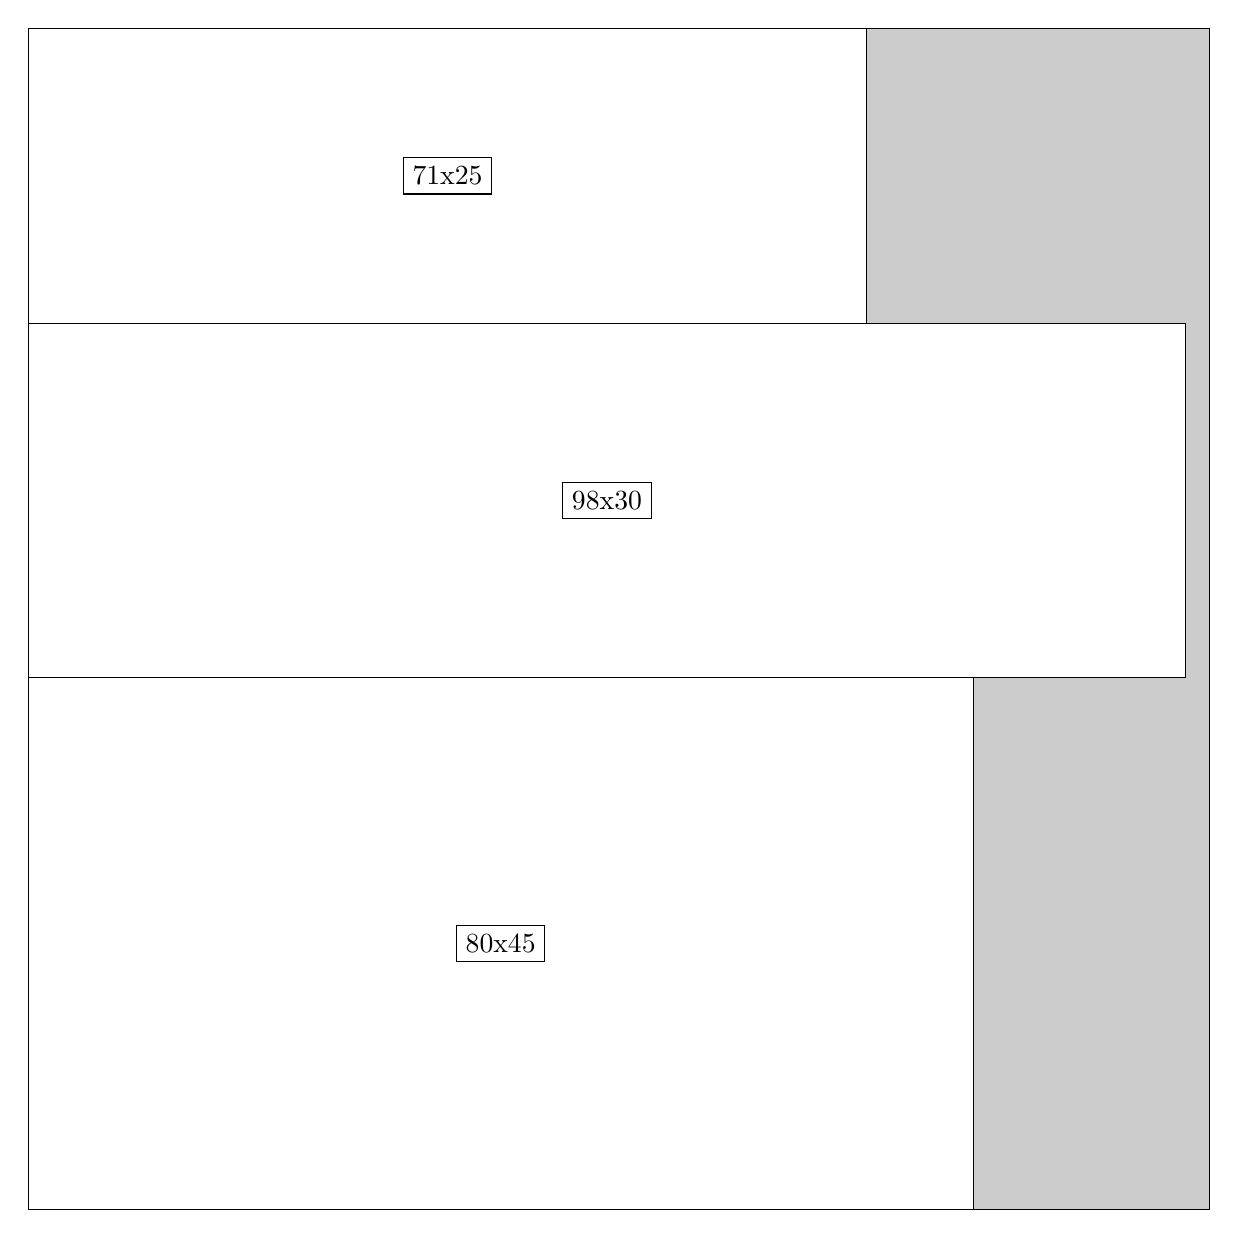
\begin{tikzpicture}[shorten >=1pt,scale=1.0,every node/.style={scale=1.0},->]
\tikzstyle{vertex}=[circle,fill=black!25,minimum size=14pt,inner sep=0pt]
\filldraw[fill=gray!40!white, draw=black] (0,0) rectangle (15.0,15.0);
\foreach \name/\x/\y/\w/\h in {80x45/0.0/0.0/12.0/6.75,98x30/0.0/6.75/14.7/4.5,71x25/0.0/11.25/10.65/3.75}
\filldraw[fill=white!40!white, draw=black] (\x,\y) rectangle node[draw] (\name) {\name} ++(\w,\h);
\end{tikzpicture}


w =80 , h =45 , x =0 , y =0 , v =3600
\par
w =98 , h =30 , x =0 , y =45 , v =2940
\par
w =71 , h =25 , x =0 , y =75 , v =1775
\par
\newpage


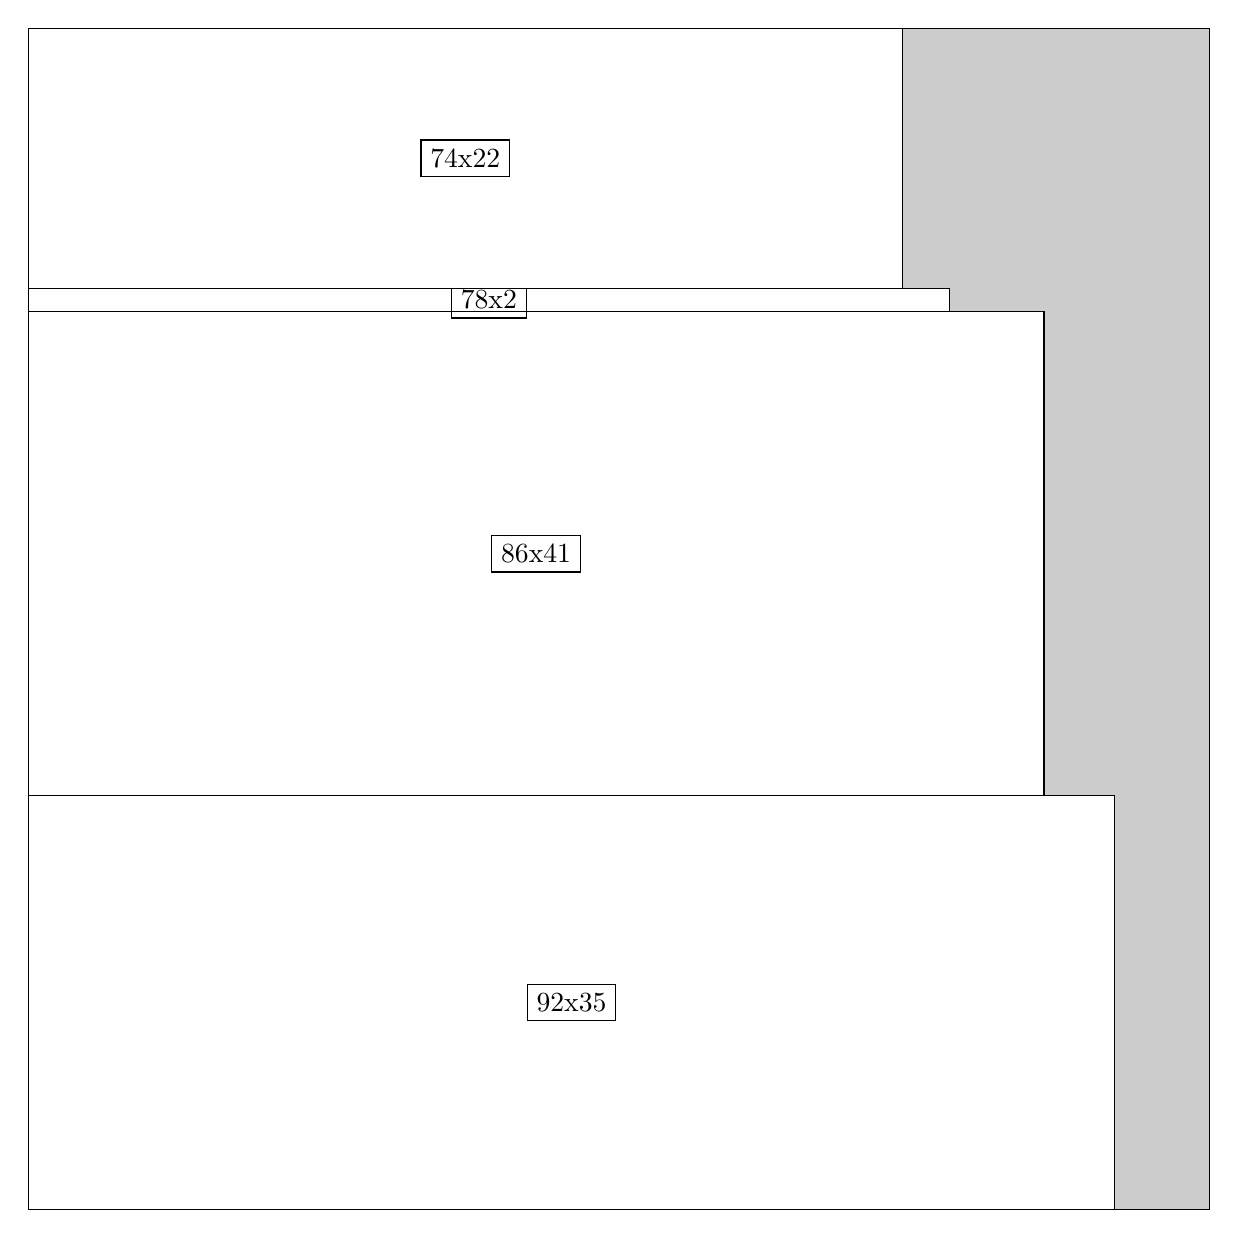
\begin{tikzpicture}[shorten >=1pt,scale=1.0,every node/.style={scale=1.0},->]
\tikzstyle{vertex}=[circle,fill=black!25,minimum size=14pt,inner sep=0pt]
\filldraw[fill=gray!40!white, draw=black] (0,0) rectangle (15.0,15.0);
\foreach \name/\x/\y/\w/\h in {86x41/0.0/5.25/12.9/6.1499999999999995,92x35/0.0/0.0/13.799999999999999/5.25,78x2/0.0/11.4/11.7/0.3,74x22/0.0/11.7/11.1/3.3}
\filldraw[fill=white!40!white, draw=black] (\x,\y) rectangle node[draw] (\name) {\name} ++(\w,\h);
\end{tikzpicture}


w =86 , h =41 , x =0 , y =35 , v =3526
\par
w =92 , h =35 , x =0 , y =0 , v =3220
\par
w =78 , h =2 , x =0 , y =76 , v =156
\par
w =74 , h =22 , x =0 , y =78 , v =1628
\par
\newpage


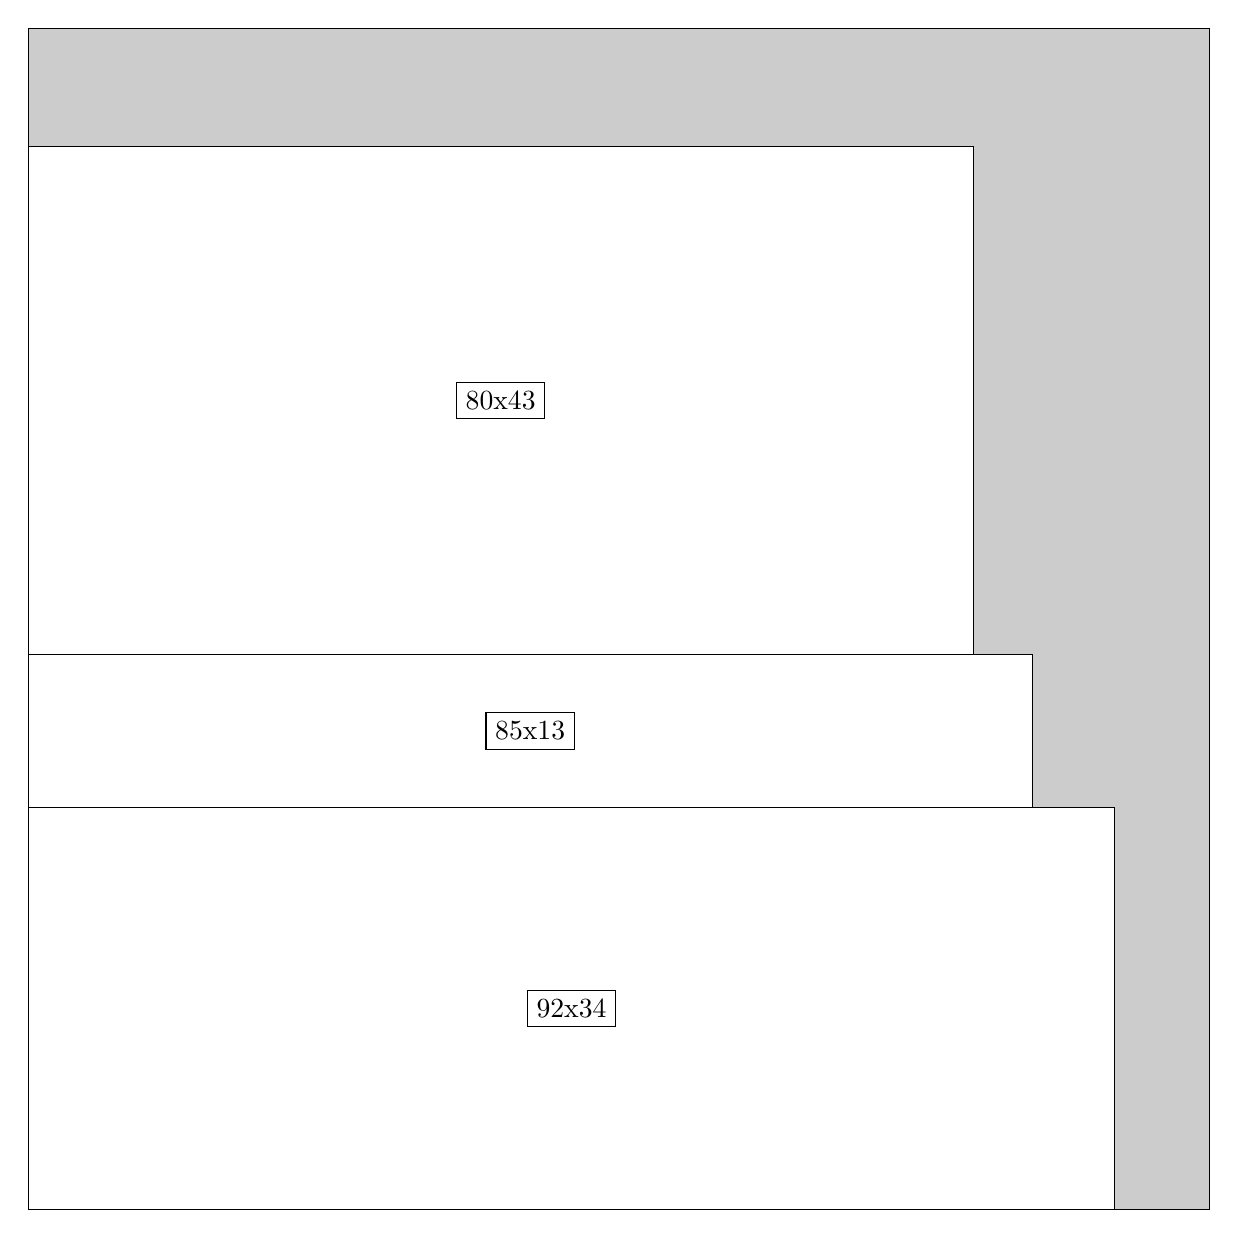
\begin{tikzpicture}[shorten >=1pt,scale=1.0,every node/.style={scale=1.0},->]
\tikzstyle{vertex}=[circle,fill=black!25,minimum size=14pt,inner sep=0pt]
\filldraw[fill=gray!40!white, draw=black] (0,0) rectangle (15.0,15.0);
\foreach \name/\x/\y/\w/\h in {80x43/0.0/7.05/12.0/6.45,92x34/0.0/0.0/13.799999999999999/5.1,85x13/0.0/5.1/12.75/1.95}
\filldraw[fill=white!40!white, draw=black] (\x,\y) rectangle node[draw] (\name) {\name} ++(\w,\h);
\end{tikzpicture}


w =80 , h =43 , x =0 , y =47 , v =3440
\par
w =92 , h =34 , x =0 , y =0 , v =3128
\par
w =85 , h =13 , x =0 , y =34 , v =1105
\par
\newpage


\end{document}